%%%%%%%%%%%%%%%%%%%%%%%%%%%%%%%%%%%%%%%%%%%%%%%%%%%%%
\section{Analyses at 100 TeV FCC-hh}
\label{sec:ana100tev}

%%%%%%%%%%%%%%%%%%%%%%%%%%%%%%%%%%%%%%%%%%%%%%%%%%%%%
%%%%%%%%%%%%%%%%%%%%%%%%%%%%%%%%%%%%%%%%%%%%%%%%%%%%%
\subsection{Leptonic resonances : ee, \texorpdfstring{$\mu\mu$}{uu}, \texorpdfstring{$\tau\tau$}{tt}}
\label{subsec:lepreso}

%%%%%%%%%%%%%%%%%%%%%%%%%%%%%%%%%%%%%%%%%%%%%%%%%%%%%%%%%%%%%%%%%%%%%%%%%%%%%%%%%%%%%%%%%%%%
\subsubsection{Introduction}
Models with extended gauge groups often feature additional U(1) symmetries with corresponding heavy spin-1 bosons. These bosons, generally referred to as $\Zp$, would manifest themselves as a narrow resonance in the dilepton mass spectrum. Among these models are those inspired by Grand Unified Theories, motivated by gauge unification or a restoration of the left-right symmetry violated by the weak interaction. Examples include the $\Zp$ bosons of the E6 motivated theories~\cite{London:1986jz,Joglekar:2016yap,Langacker:2008yv,Hewett:1988xc} and Minimal models~\cite{Salvioni:2009mt}. The Sequential Standard Model (SSM)~\cite{Langacker:2008yv} posits a $\ZpSSM$ boson with couplings to fermions that are identical to those of the Standard Model $\Z$ boson.

The decay products of heavy resonances are in the multi-TeV regime and the capability to reconstruct their momentum imposes stringent requirement on the detector design. In particular, reconstructing the track curvature of multi-TeV muons requires excellent position resolution and a large lever arm. In this section, the expected sensitivity is presented for a \Zpll\ (where $\ell=\mathrm{e},\mu$) and \Zptata\ separately.

%%%%%%%%%%%%%%%%%%%%%%%%%%%%%%%%%%%%%%%%%%%%%%%%%%%%%%%%%%%%%%%%%%%%%%%%%%%%%%%%%%%%%%%%%%%%
\subsubsection{Event Selection}
Events are required to contain two leptons with $\pt > 1$~TeV, $|\eta|$<4 and an invariant mass $\mll > 2.5$~TeV. For di-$\tau$ final state we focus on the most sensitive fully hadronic channel only. The di-$\tau$ event selection requires two jets with $p_{T} > 0.5$>~TeV and $|\eta|<2.5$ identified as $\tau$'s. To ensure no overlap between the $\ell$ and $\tau$ final states, jets containing leptons with $\pt > 100$~GeV are vetoed. Finally, requirements of $\Delta \phi(\tau_1, \tau_2)> 2$ and $2.5<\Delta R(\tau_1, \tau_2)<4$ are applied.
Mass dependent cuts applied to maximise the signal to background ratio are summarised in Table~\ref{tab:leptonicresonances:selectiontautau}.

Figure~\ref{figure:leptonicresonances:masses} (left and center) shows the invariant mass for a 30~TeV signal for the $ee$ and $\mu\mu$ channels, and the yields can be found in Table~\ref{tab:leptonicresonances:yieldstautau}. The mass resolution is better for the ee channel, as expected. Figure~\ref{figure:leptonicresonances:masses} (right) shows the transverse mass~\footnote{the transverse mass is defined as $m_{T}  =  \sqrt{2\ptZp*\met*(1-cos\Delta\phi(\Zp,\met))} $}
of a 10~TeV signal for the $\tau\tau$ channel, and the yields can be found in Table~\ref{tab:leptonicresonances:yieldsll}.
Several proxies for the true resonance mass have been tested, such as the invariant mass of the two taus, with and without correction for the missing energy. The transverse mass provided the best sensitivity and was therefore used to set limits and determine the discovery reach.

\begin{table}[htbp]
   \centering
\begin{tabular}{|l|l|c|r|}
  \hline
  \hline
   $\Zp$ mass [TeV] &  $\Delta \phi(\tau_1, \tau_2)$&  $\Delta R(\tau_1, \tau_2)$ & $\met$\\
  \hline
  $4-8$ & > 2.4 & > 2.5 and < 3.5 & > 400 GeV\\
  $10$ & > 2.4 & > 2.7 and < 4 & > 300 GeV\\
  $12-14$ & > 2.6 & > 2.7 and < 4 & > 300 GeV\\
  $16-18$ & > 2.7 & > 2.7 and < 4 & > 300 GeV\\
  $>18$ & > 2.8 & > 3 and < 4 & > 300 GeV\\
  \hline
  \hline
  \end{tabular}
  \caption{List of mass dependent cuts optimised to maximise the sensitivity for the \Zptata\ search.}
  \label{tab:leptonicresonances:selectiontautau}
\end{table}

\begin{table}[htbp]
   \centering
\begin{tabular}{|l|r|r|}
  \hline
  \hline
 & ee & $\mu\mu$  \\
  \hline
  Drell-Yan & 206882.9 & 236597.9 \\
  \hline
  $\Zp$ 4~TeV & 1421357.9    & 1598969.4 \\
  $\Zp$ 6~TeV & 349922.4  & 393117.6\\
  $\Zp$ 8~TeV &   115043.5 & 129698.7 \\
  $\Zp$ 10~TeV &  45423.5 & 50873.3 \\
  $\Zp$ 20~TeV &  1192.3 & 1411.5\\
  $\Zp$ 30~TeV &  88.2 & 107.6\\
  $\Zp$ 40~TeV &  11.7 & 14.1 \\
  $\Zp$ 50~TeV &  3.2 & 3.7\\
  \hline
  \hline
\end{tabular}
  \caption{Expected number of events for the \Zpee\ and \Zpmumu\ analysis after the full event selection for the various \Zp\ mass hypotheses}
  \label{tab:leptonicresonances:yieldsll}
\end{table}

\begin{table}[htbp]
   \centering
\begin{tabular}{|l|r|r|r|}
  \hline
  \hline
$\Zp$ mass [TeV]  & signal &  Drell-Yan & Di-jet \\
  \hline
  $4$     &  51479.5 &  \multirow{3}{*}{5669.2} &   \multirow{3}{*}{875561.7} \\
  $6$     &  22294.3  & &\\
  $8$     &  9140.7  &  &\\
  \hline

  $10$      & 5398.8 & 9008.3 & 2040422.6 \\
  \hline

  $12$ &  2261.4&  \multirow{3}{*}{8946.8} &  \multirow{3}{*}{1982792.8}  \\
  $14$ &  1040.9&  &  \\
  \hline

  $16$ &  489.6&  \multirow{3}{*}{8826.3} &  \multirow{3}{*}{1915211.5} \\
  $18$ &  251.9&  &  \\
    \hline

  $20$    &  122.6& \multirow{3}{*}{7777.2} & \multirow{3}{*}{1609435.6}   \\
  $25$    &  27.5 &  &  \\
  $30$    &  7.1 &  &  \\
  \hline
  \hline
\end{tabular}
  \caption{Expected number of events for the \Zptata\ analysis after the full event selection for the various \Zp\ mass hypotheses}
  \label{tab:leptonicresonances:yieldstautau}
\end{table}

\begin{figure}[!htb]
  \centering
  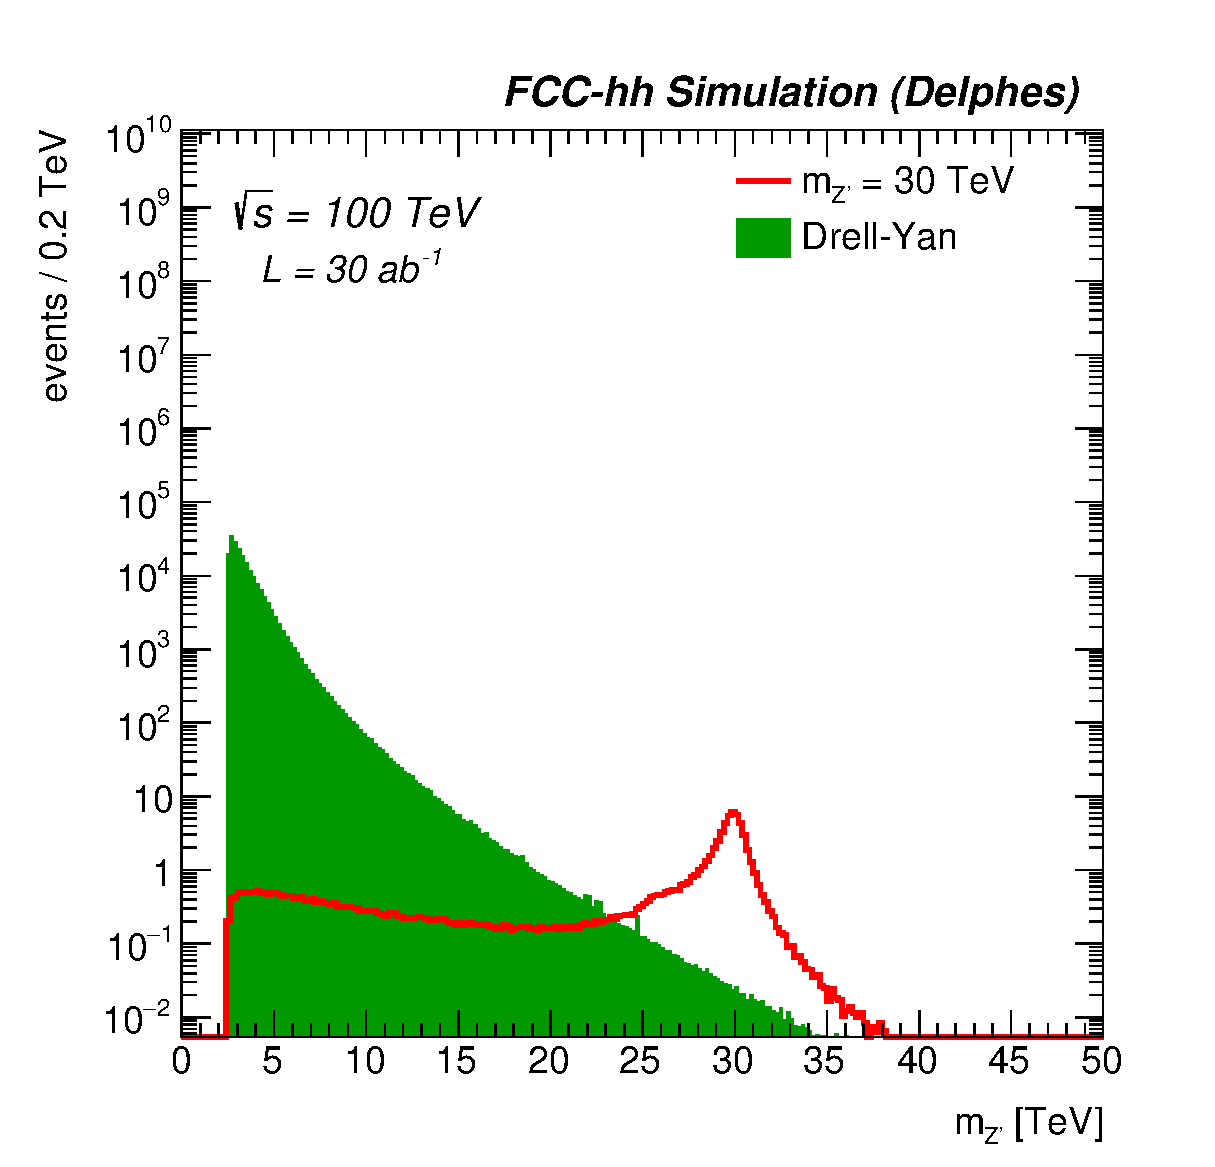
\includegraphics[width=0.32\columnwidth]{Fig/mzp_sel0_nostack_log_ee.eps}
  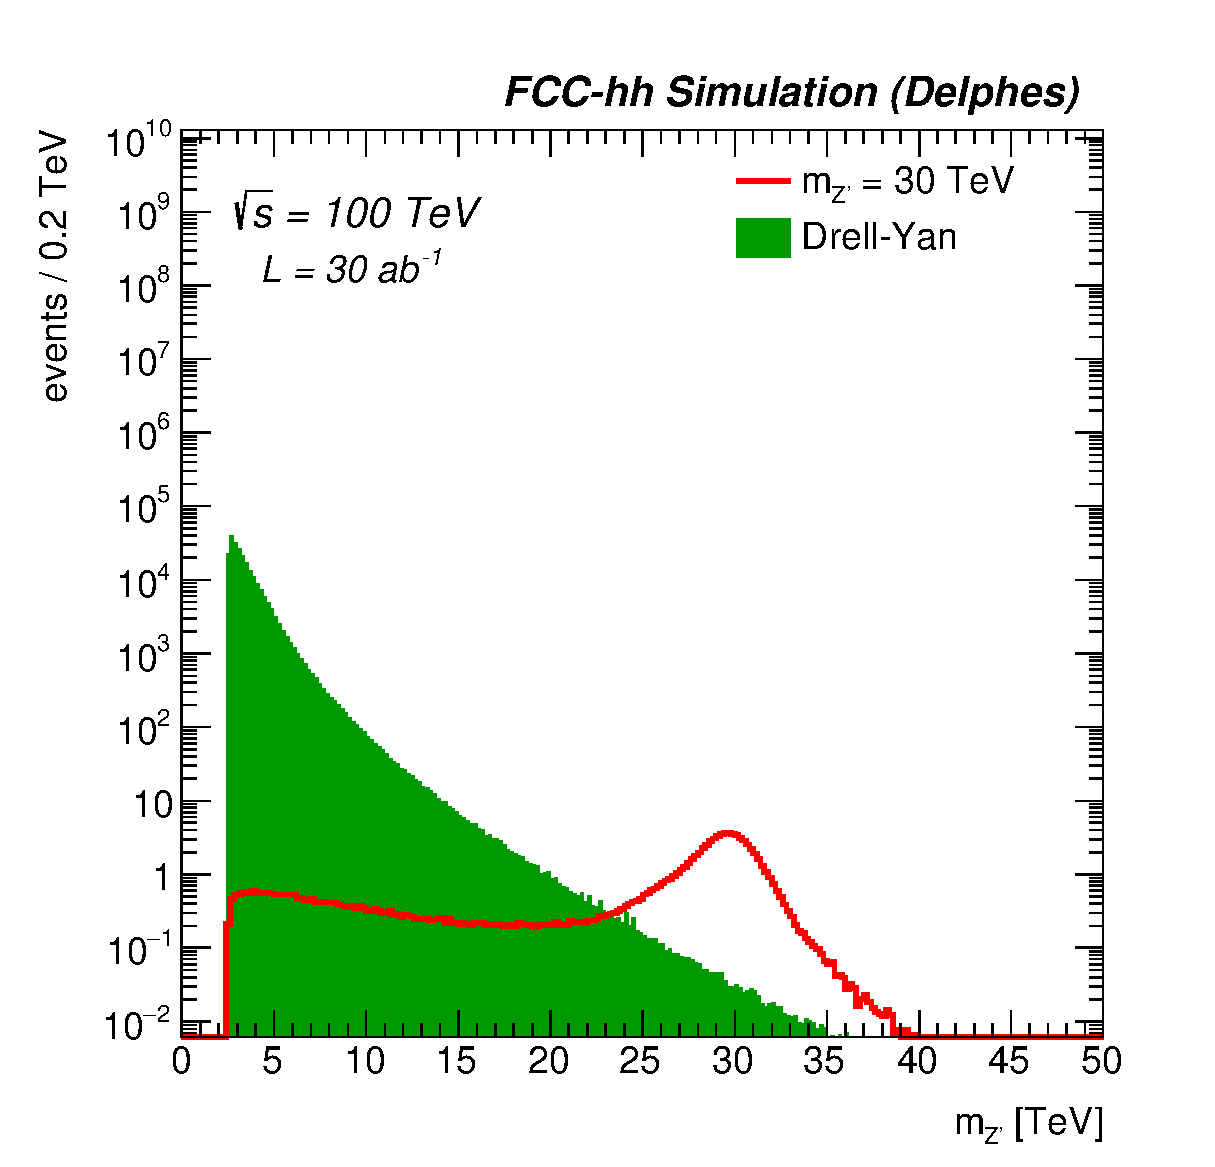
\includegraphics[width=0.32\columnwidth]{Fig/mzp_sel0_nostack_log_mm.eps}
  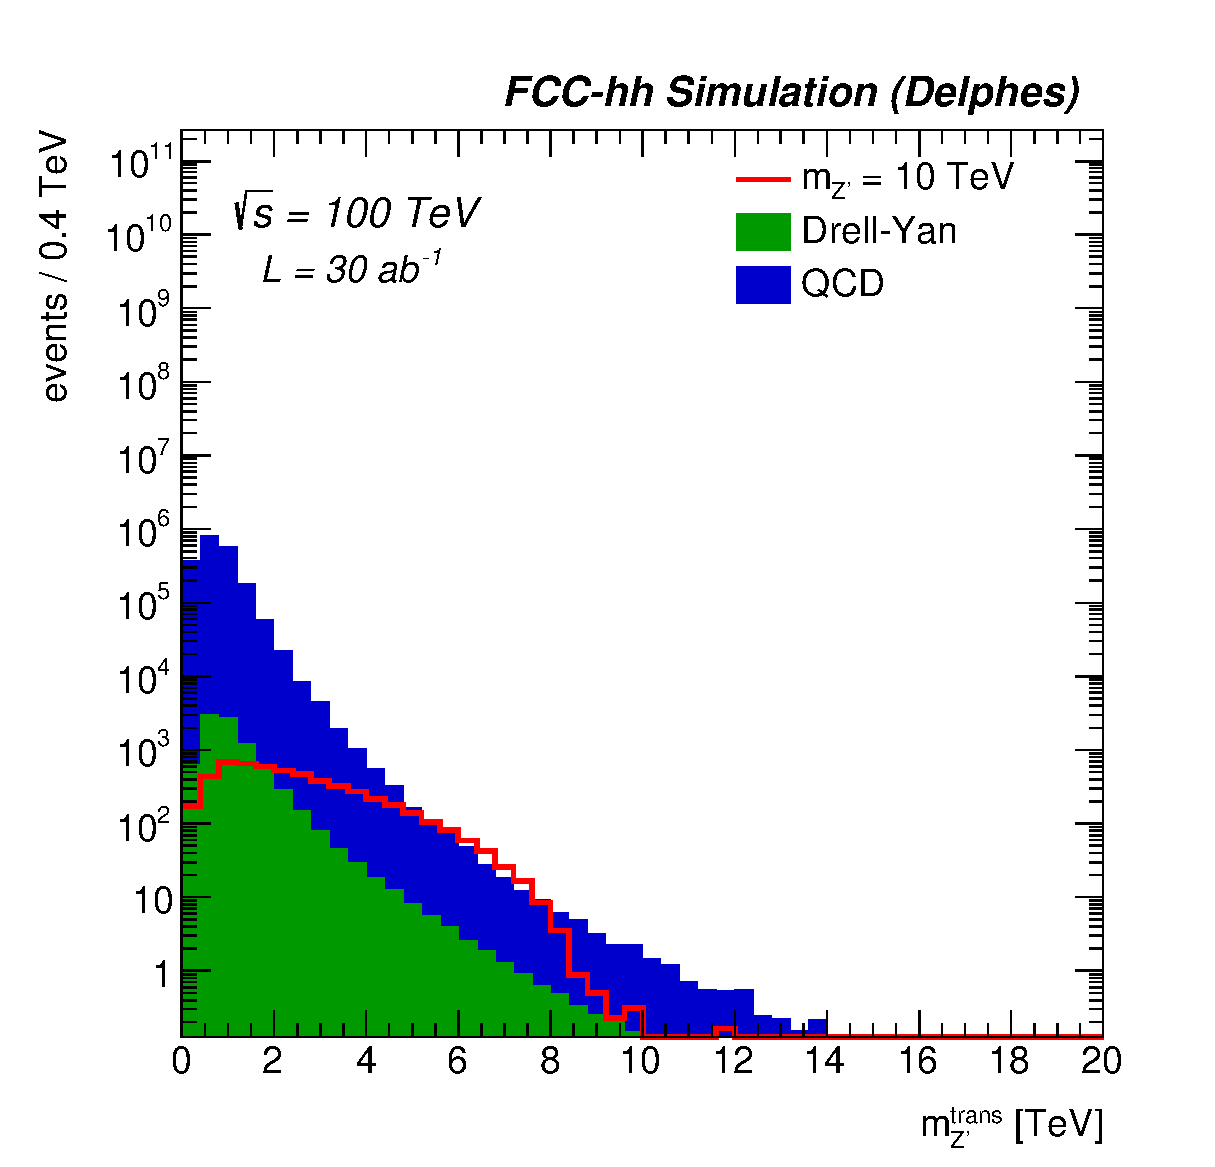
\includegraphics[width=0.32\columnwidth]{Fig/mt_finalsel_nostack_log.eps}
  \caption{Left, center: Invariant mass for a 30~TeV signal after full event selection for ee channel (left) and $\mu\mu$ channel (center). Right: Transverse mass for a 10~TeV signal after full event selection for the $\tau\tau$ channel. }
  \label{figure:leptonicresonances:masses}
\end{figure}
%\MS{need editing / style}

%%%%%%%%%%%%%%%%%%%%%%%%%%%%%%%%%%%%%%%%%%%%%%%%%%%%%%%%%%%%%%%%%%%%%%%%%%%%%%%%%%%%%%%%%%%%
\subsubsection{Results and discussion}
Hypothesis testing is performed using a modified frequentist method based on a profile likelihood that takes into account the systematic uncertainties as nuisance parameters that are fitted to the expected Monte-Carlo. For the $ee$ and $\mu\mu$ analyses, the di-lepton invariant mass is used as the discriminant, while for the $\tau\tau$ channel the transverse mass is used. A 50\% uncertainty on the background normalisation is assumed.

Figure~\ref{figure:leptonicresonances:resultsll} shows the exclusion limit obtained \intlumifcc\ of data for the ee alone (top left), $\mu\mu$ alone (top right) and combination of (ee,$\mu\mu$) channels (bottom left). Figure~\ref{figure:leptonicresonances:resultsll} (bottom right) shows the integrated luminosity required to reach a $5\sigma$ discovery for the leptonic resonances as a function of the mass of the heavy resonance. The \Zpee\ and \Zpmumu\ channel display very similar performance, due to the low background rates. We conclude therefore that the reference detector design features near to optimal performance for searches involving high \pT\ muon final states. Figure~\ref{figure:leptonicresonances:resultstautau} shows the exclusion limits for 30 ab$^{-1}$ of data (left) and the required integrated luminosity
versus mass to reach a $5\sigma$ discovery (right) for the di-tau resonances.

The discovery potential for high mass resonances decaying to $ee$, $\mu\mu$ and $\tau\tau$ has been studied using as a benchmark the \ZpSSM\ model. The very large centre of mass energy provides a correspondingly large mass reach. For the $ee$ and $\mu\mu$ cases masses up to 42~TeV can be excluded or discovered. Heavy resonance decaying to $\tau$ leptons reconstructed in the hadronic decay mode are more challenging, but we would be able to probe massses up to 18~TeV.

\begin{figure}[!htb]
  \centering
  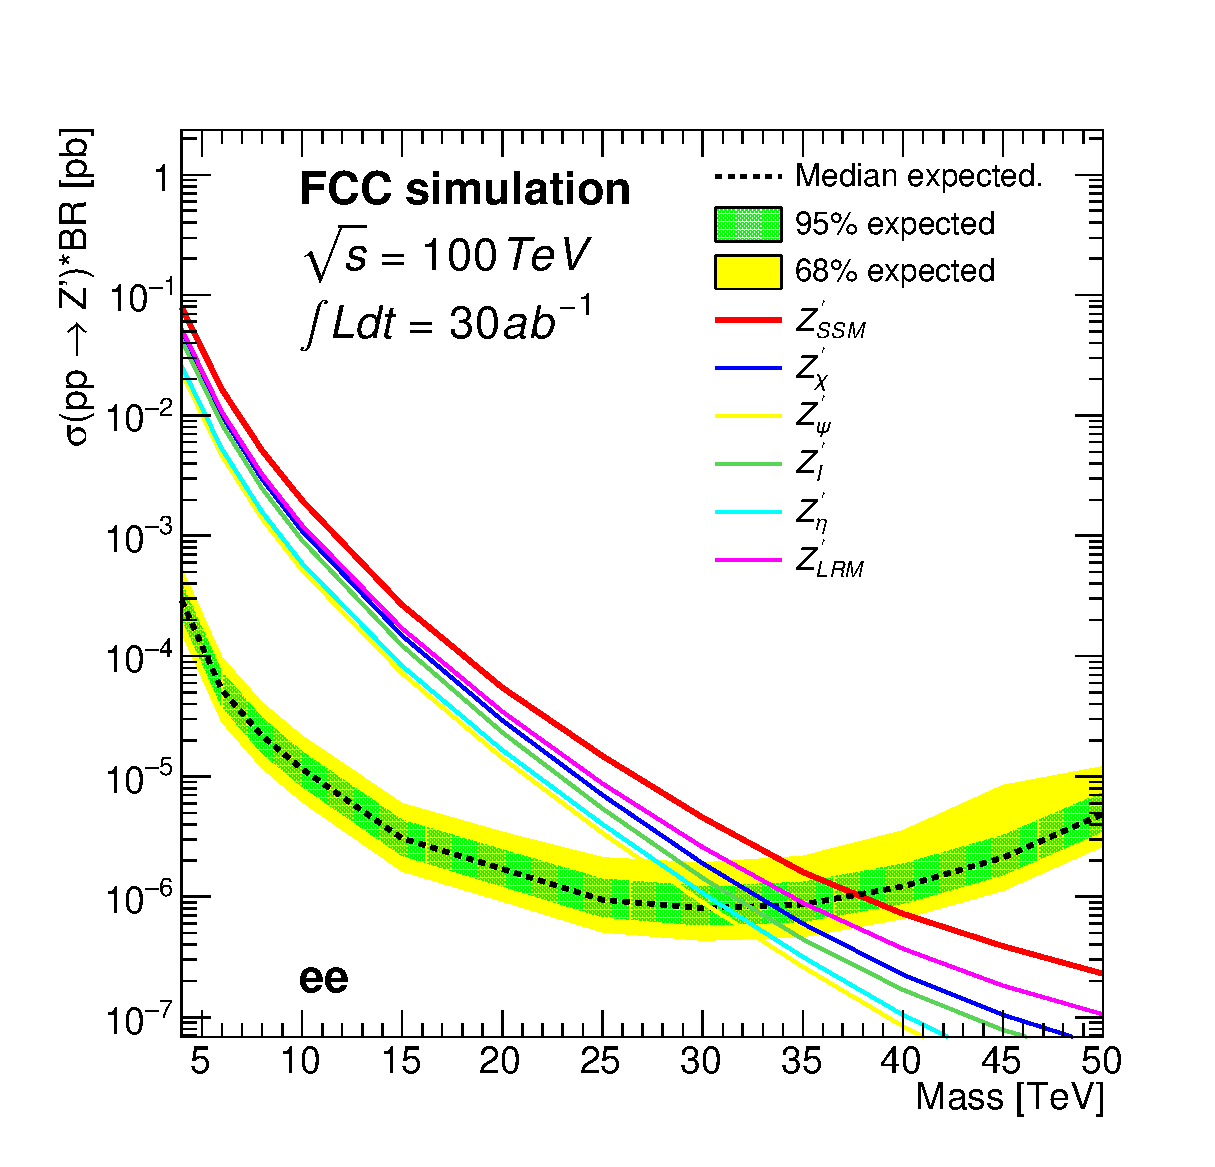
\includegraphics[width=0.33\columnwidth]{Fig/lim_Zprime_ee_fcc_v02_allxs.eps}
  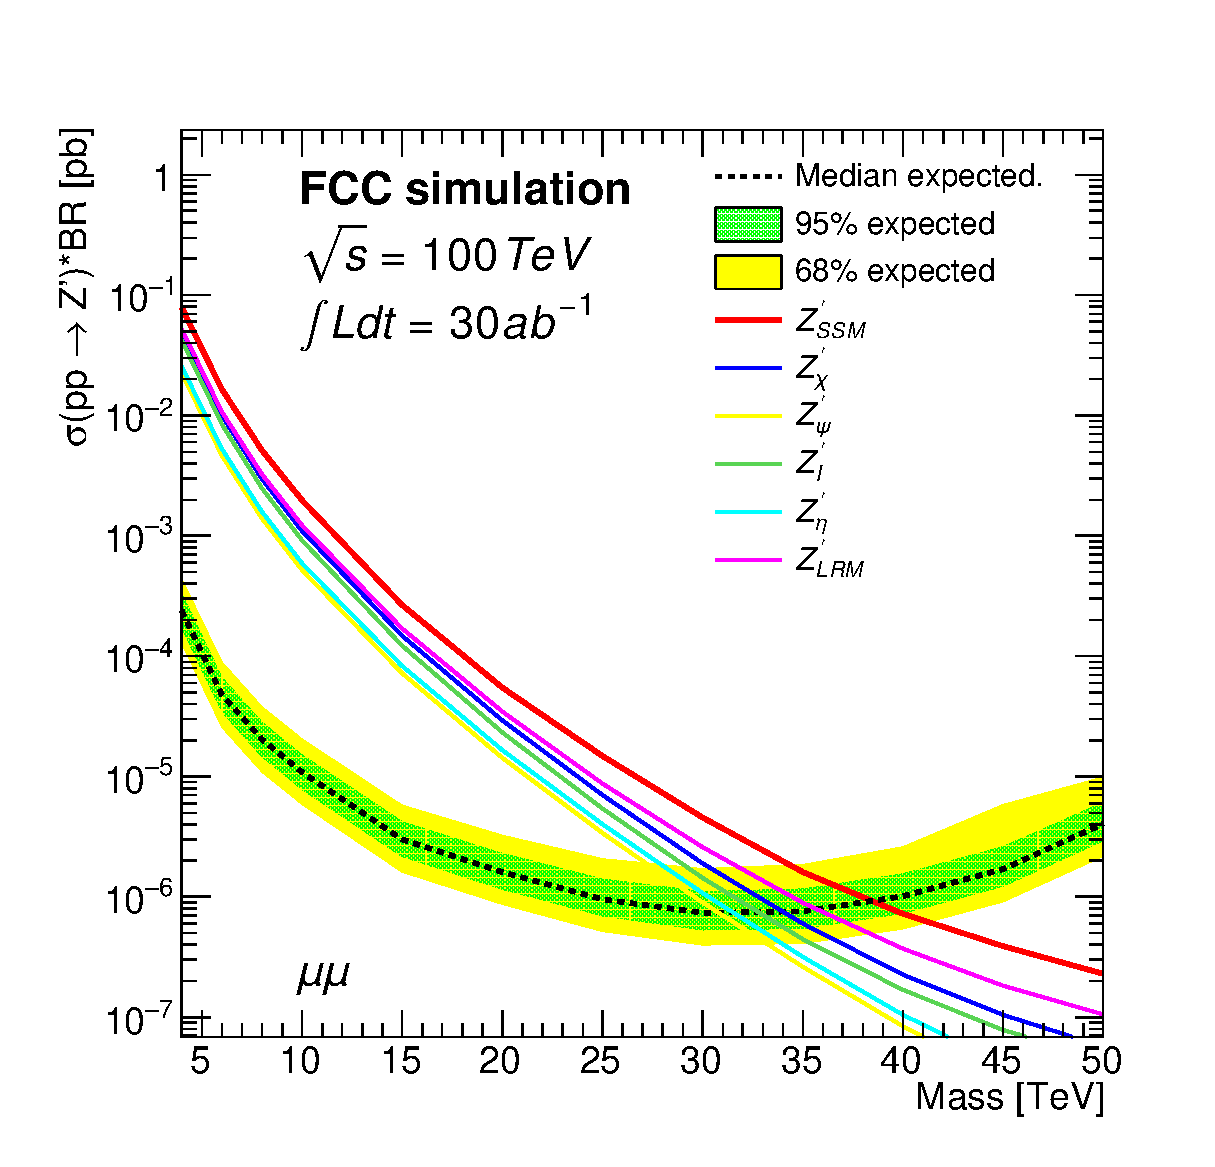
\includegraphics[width=0.33\columnwidth]{Fig/lim_Zprime_mumu_fcc_v02_allxs.eps}
  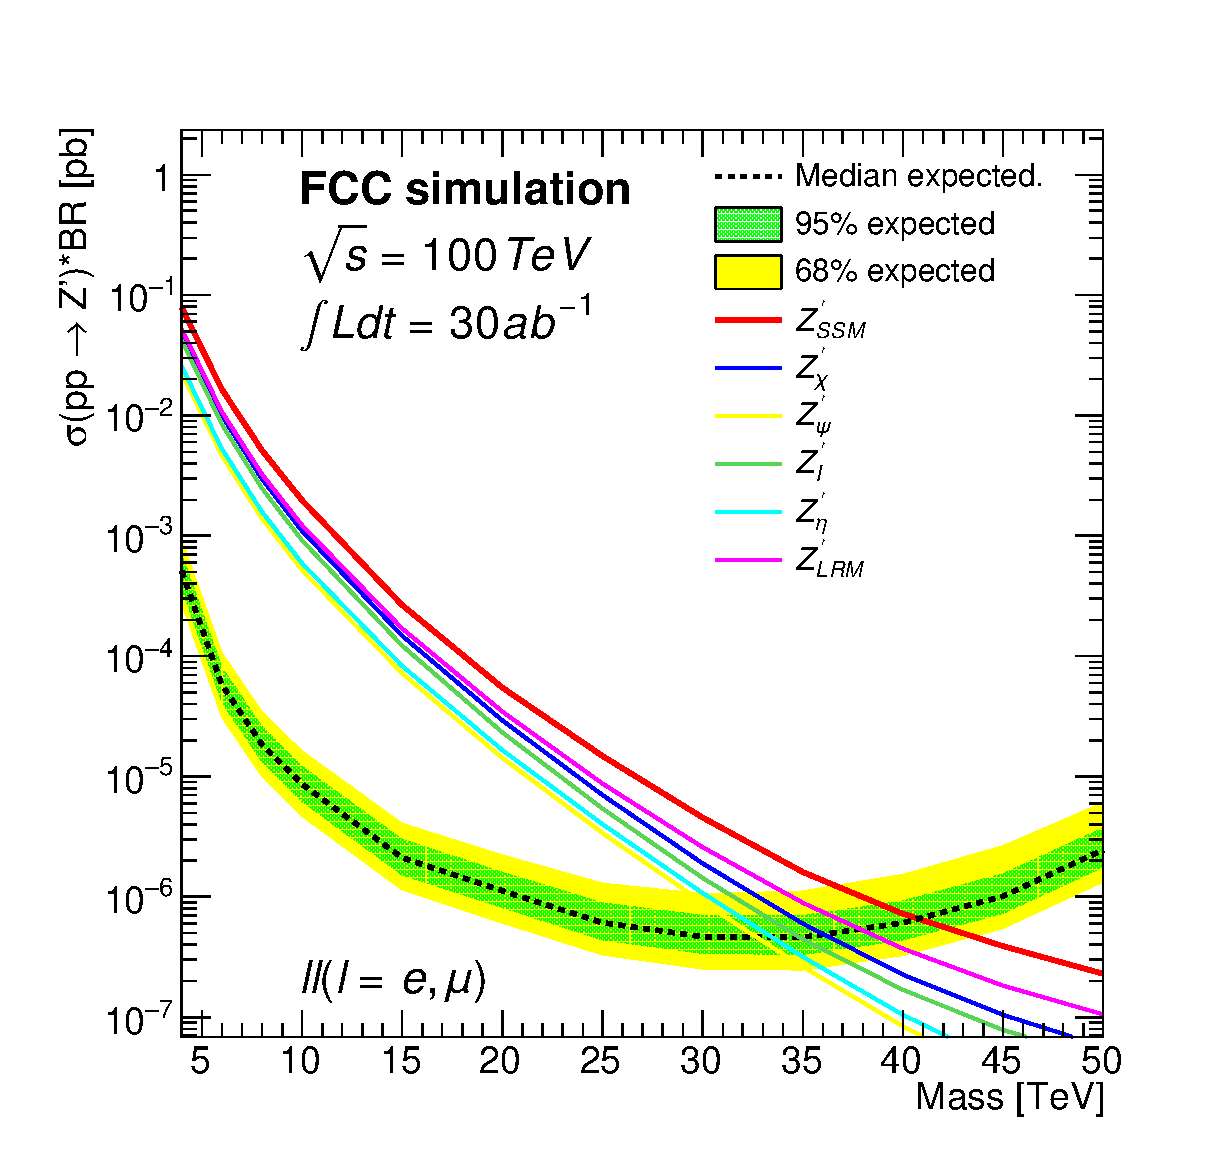
\includegraphics[width=0.33\columnwidth]{Fig/lim_Zprime_ll_fcc_v02_allxs.eps}
  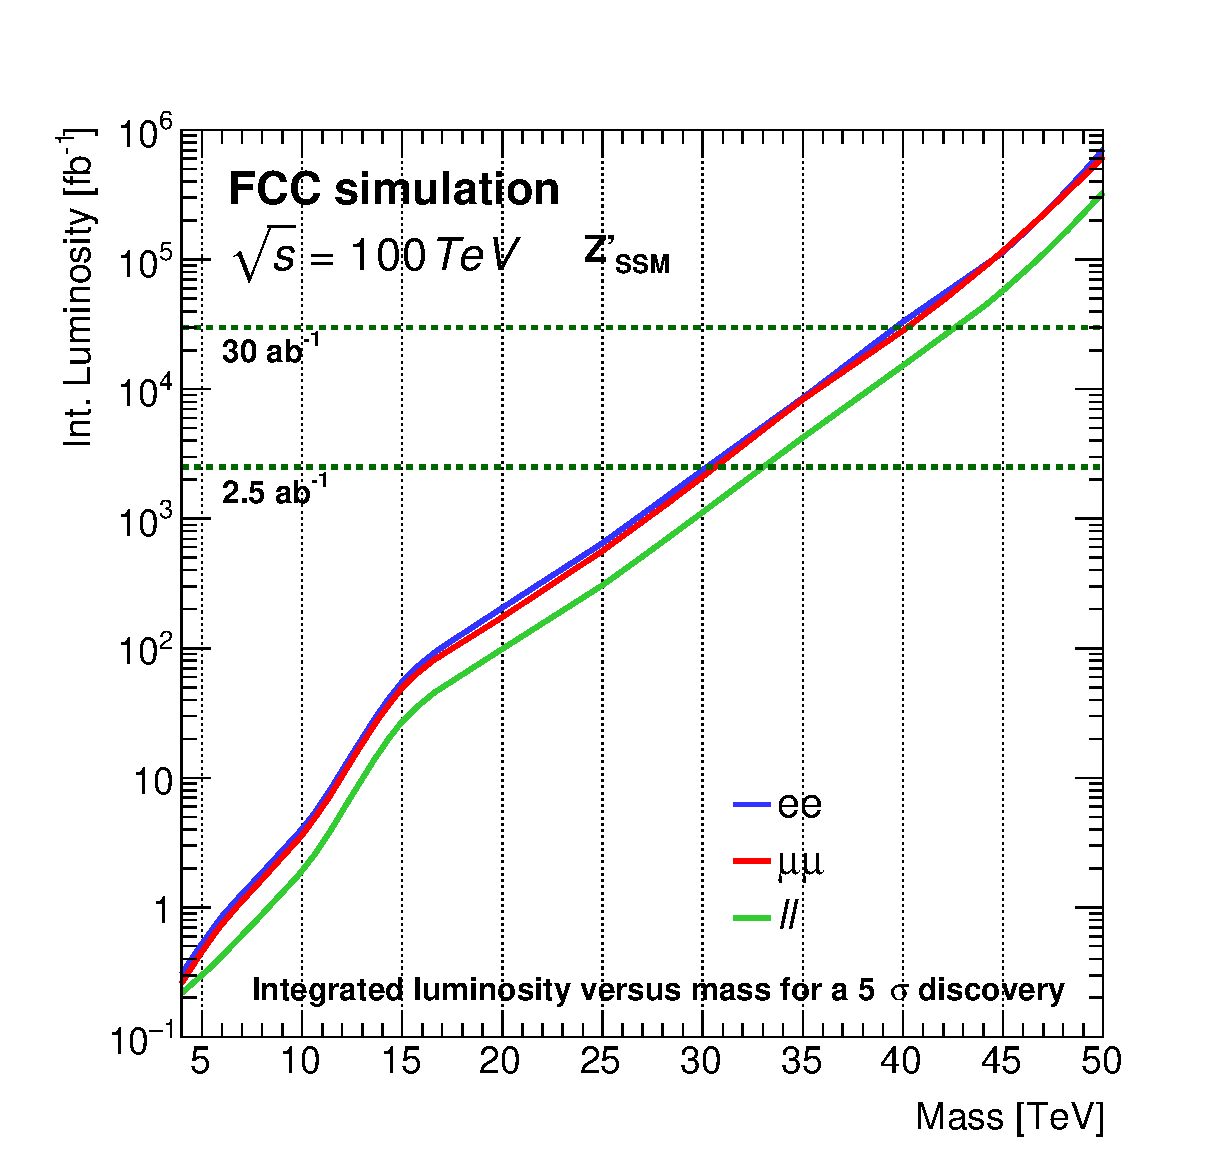
\includegraphics[width=0.33\columnwidth]{Fig/DiscoveryPotential_ll_comb_rootStyle.eps}
  \caption{Limit versus mass for the di-lepton (ee,$\mu\mu$) channel (left) and luminosity for a $5\sigma$ discovery (right) comparing ee,$\mu\mu$ and combined channels. }
  \label{figure:leptonicresonances:resultsll}
\end{figure}

\begin{figure}[!htb]
  \centering
  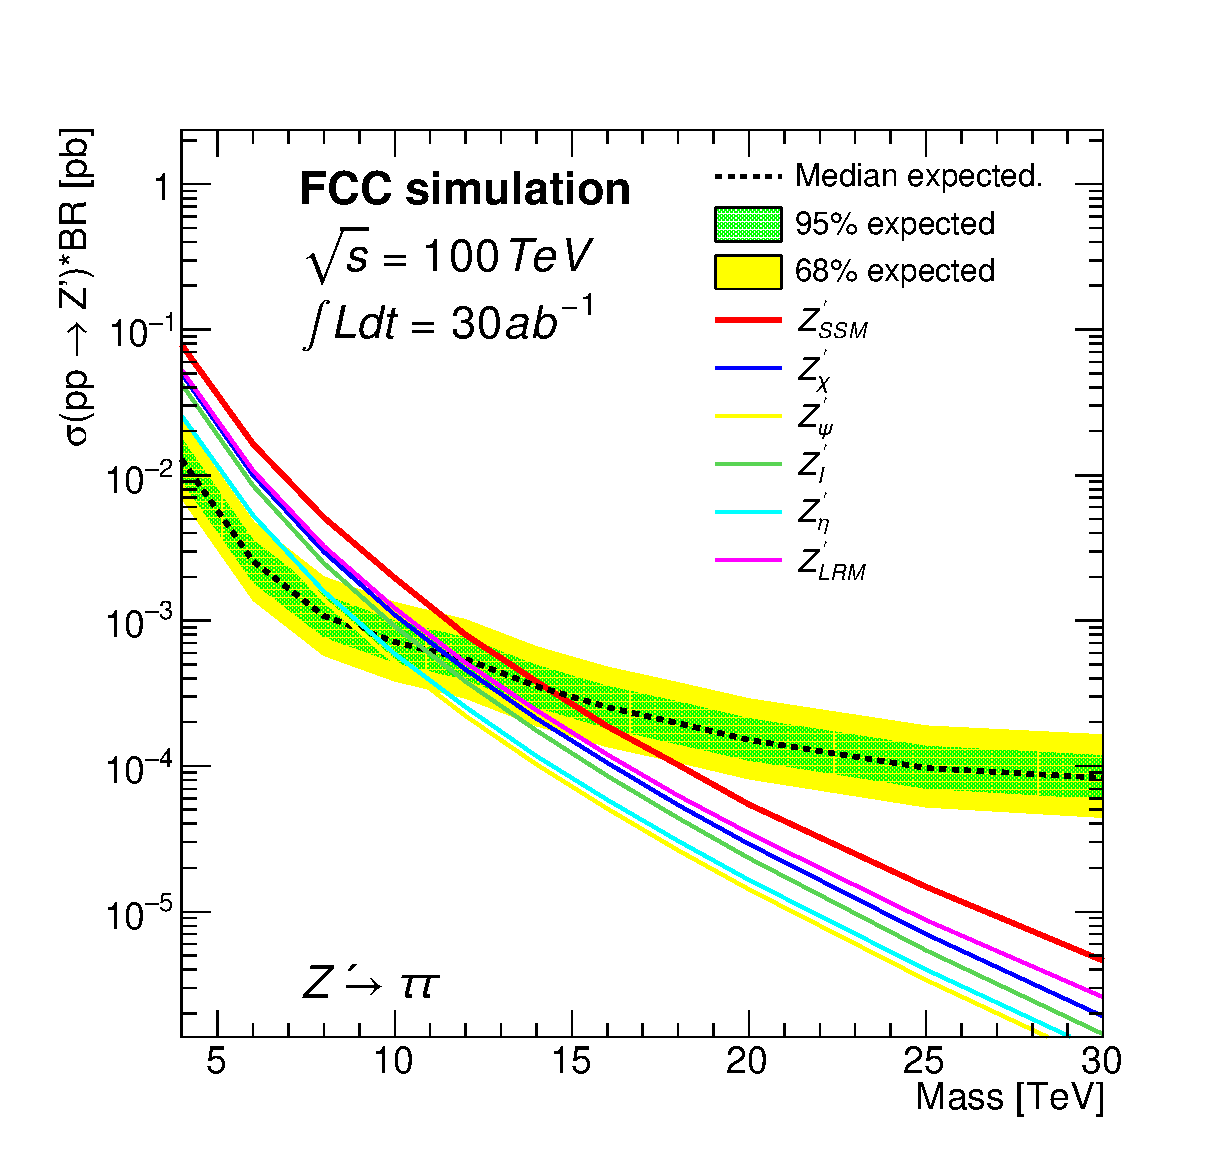
\includegraphics[width=0.33\columnwidth]{Fig/lim_Zprime_tautau_fcc_v02_allxs.eps}
  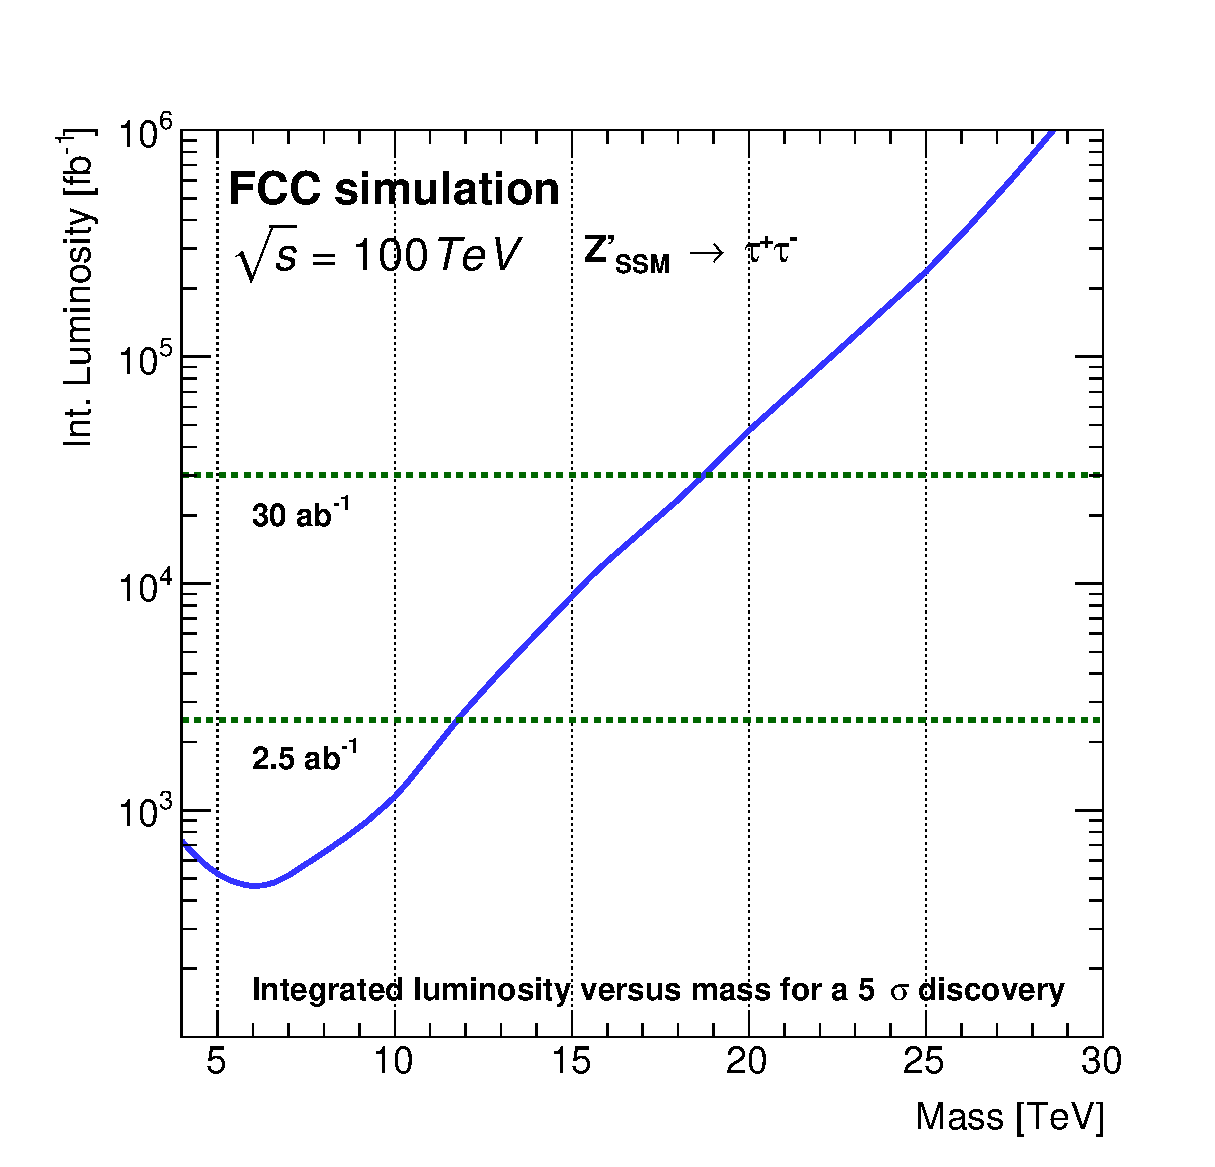
\includegraphics[width=0.33\columnwidth]{Fig/DiscoveryPotential_tautau_rootStyle.eps}
  \caption{Limit versus mass for the di-tau channel (left) and luminosity for a $5\sigma$ discovery (right). }
  \label{figure:leptonicresonances:resultstautau}
\end{figure}


\subsection{\texorpdfstring{$\mu\mu$}{uu} non-resonant interpretations}
LHCb measurements in $B\rightarrow~K^*\mu~+\mu~-$ decays are somewhat discrepant with Standard Model predictions~\cite{Aaij:2014ora,Aaij:2017vbb}. They may be harbingers of new physics at an energy scale potentially accessible to direct discovery. The flavour anomaly (f.a.) model $Z'$ and t-channel LQ interpretations from~\cite{Allanach:2017bta} are studied in this section.
\newline
The selection strategy is the same as the $Z'\rightarrow~\mu^+\mu^-$ in section~\ref{subsec:lepreso}. The only difference is the increase of lepton momentum threshold from 1 to 1.2 TeV.
\newline
Figure~\ref{figure:leptonicresonances:resultsmumu_flav} ($Z'$ f.a.) and ~\ref{figure:leptonicresonances:resultsmumu_flav} (t-channel LQ) show the invariant mass of the $\mu^+\mu^-$ system (left), the exclusion limit obtained \intlumifcc\ (middle) and the integrated luminosity required to reach a $5\sigma$ discovery for the two scenarios as a function of the mass of the $\mu^+\mu^-$ system (right).
It is found that $Z'$ is visible and LQ would need to search for pair production.

\begin{figure}[!htb]
  \centering
  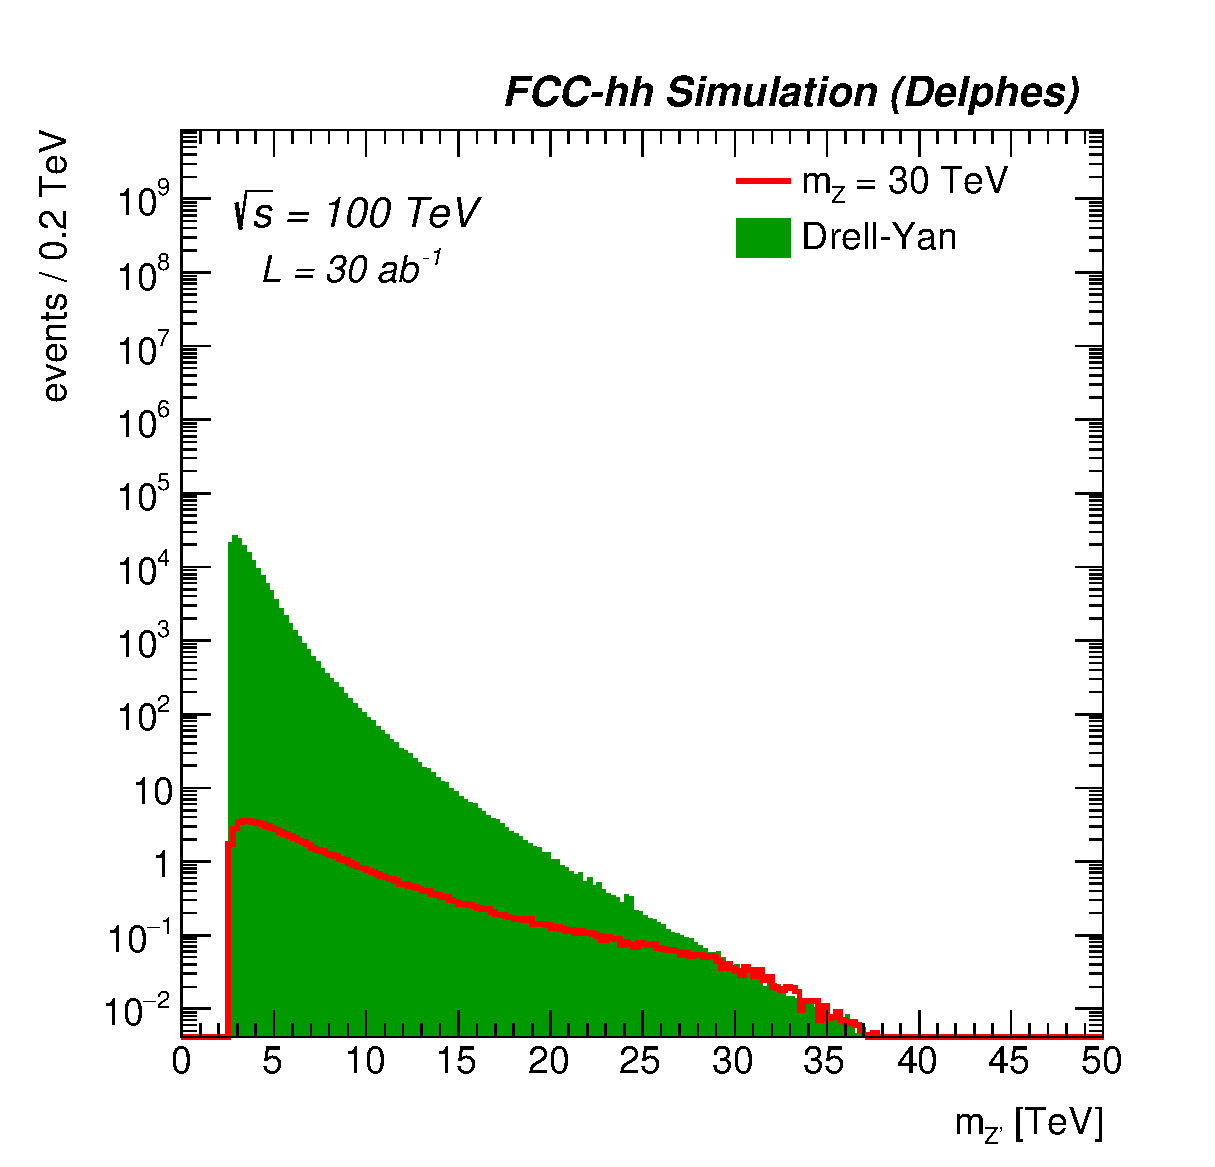
\includegraphics[width=0.32\columnwidth]{Fig/mzp_sel0_nostack_log.eps}
  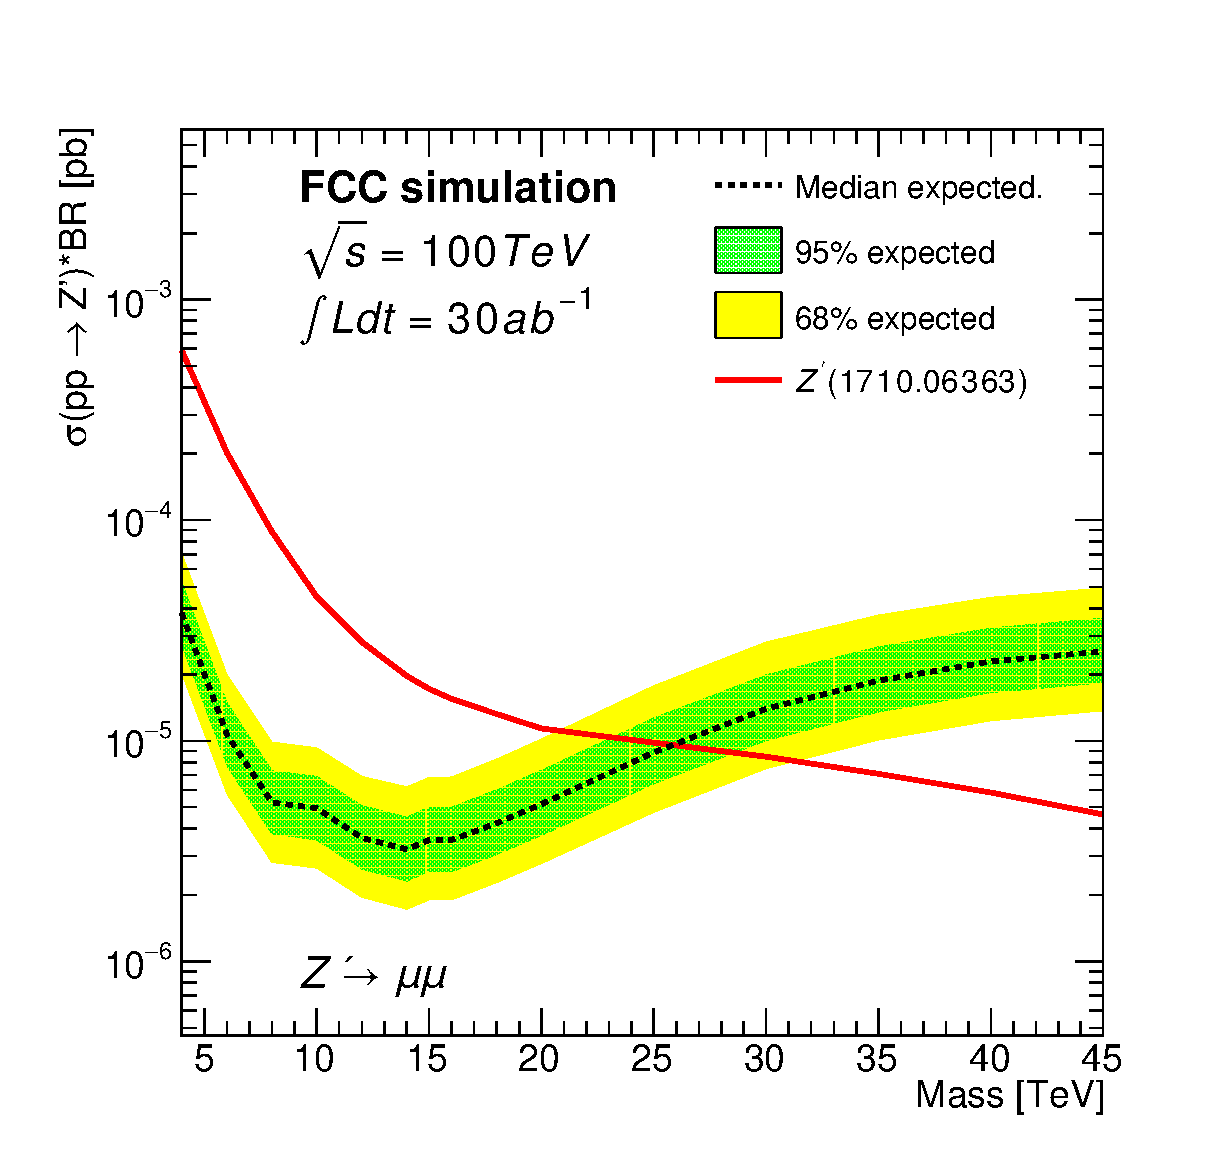
\includegraphics[width=0.32\columnwidth]{Fig/lim_Zprime_mumu_ano_fcc_v02.eps}
  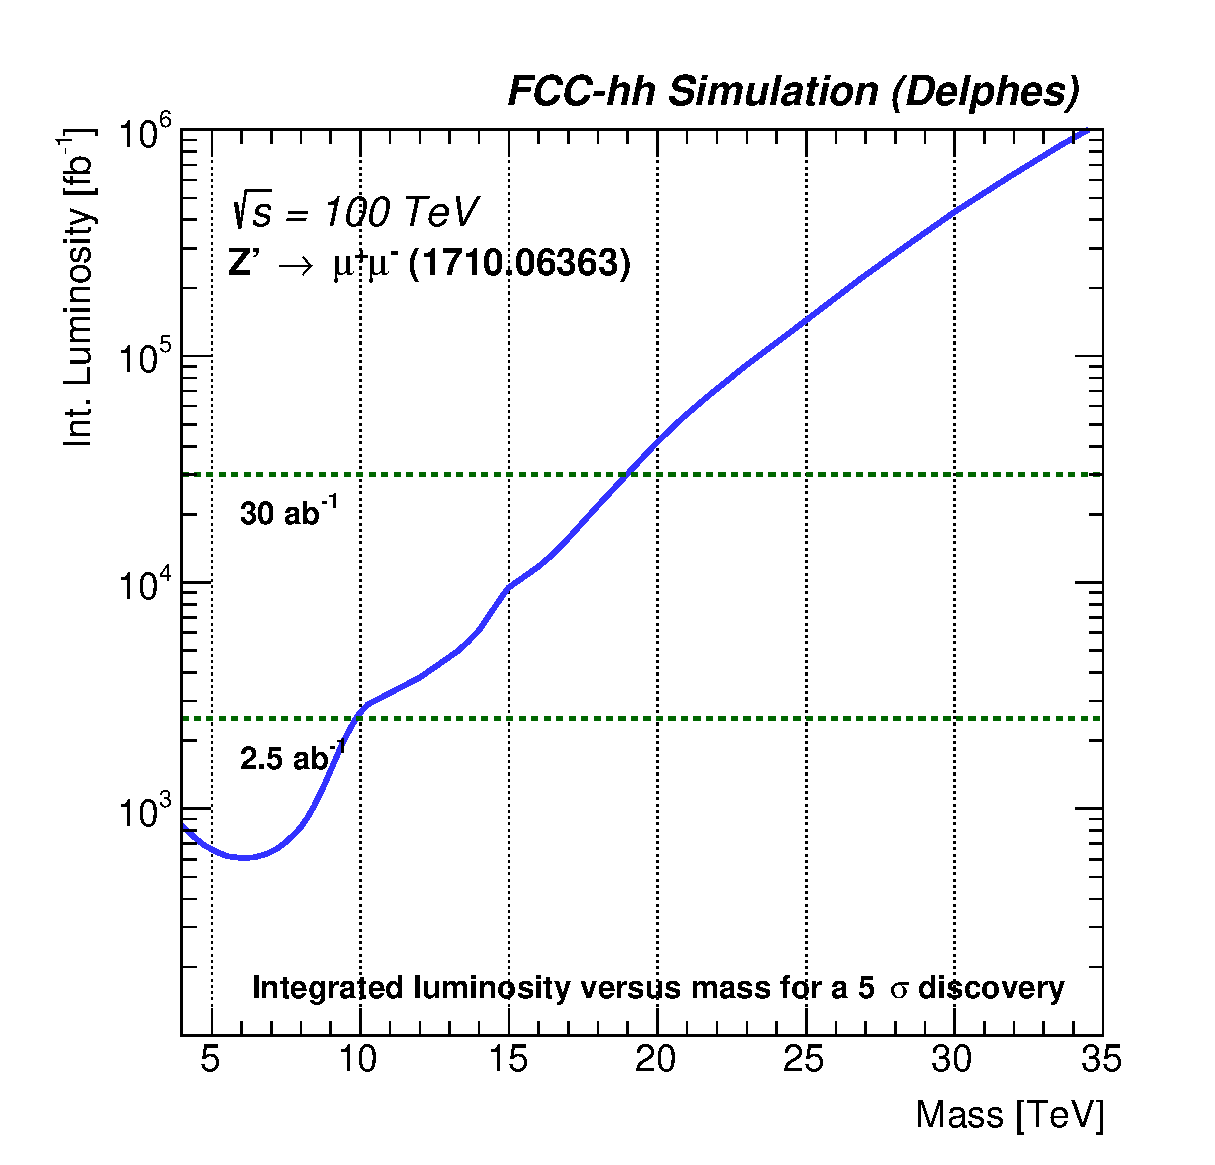
\includegraphics[width=0.32\columnwidth]{Fig/DiscoveryPotential_mumu_rootStyle.eps}
  \caption{Left : Invariant mass for a 30~TeV signal after full event selection in flavour anomaly scenario. Limit versus mass (middle) and luminosity for a $5\sigma$ discovery (right) comparing ee,$\mu\mu$ and combined channels. }
  \label{figure:leptonicresonances:resultsmumu_flav}
\end{figure}

\begin{figure}[!htb]
  \centering
  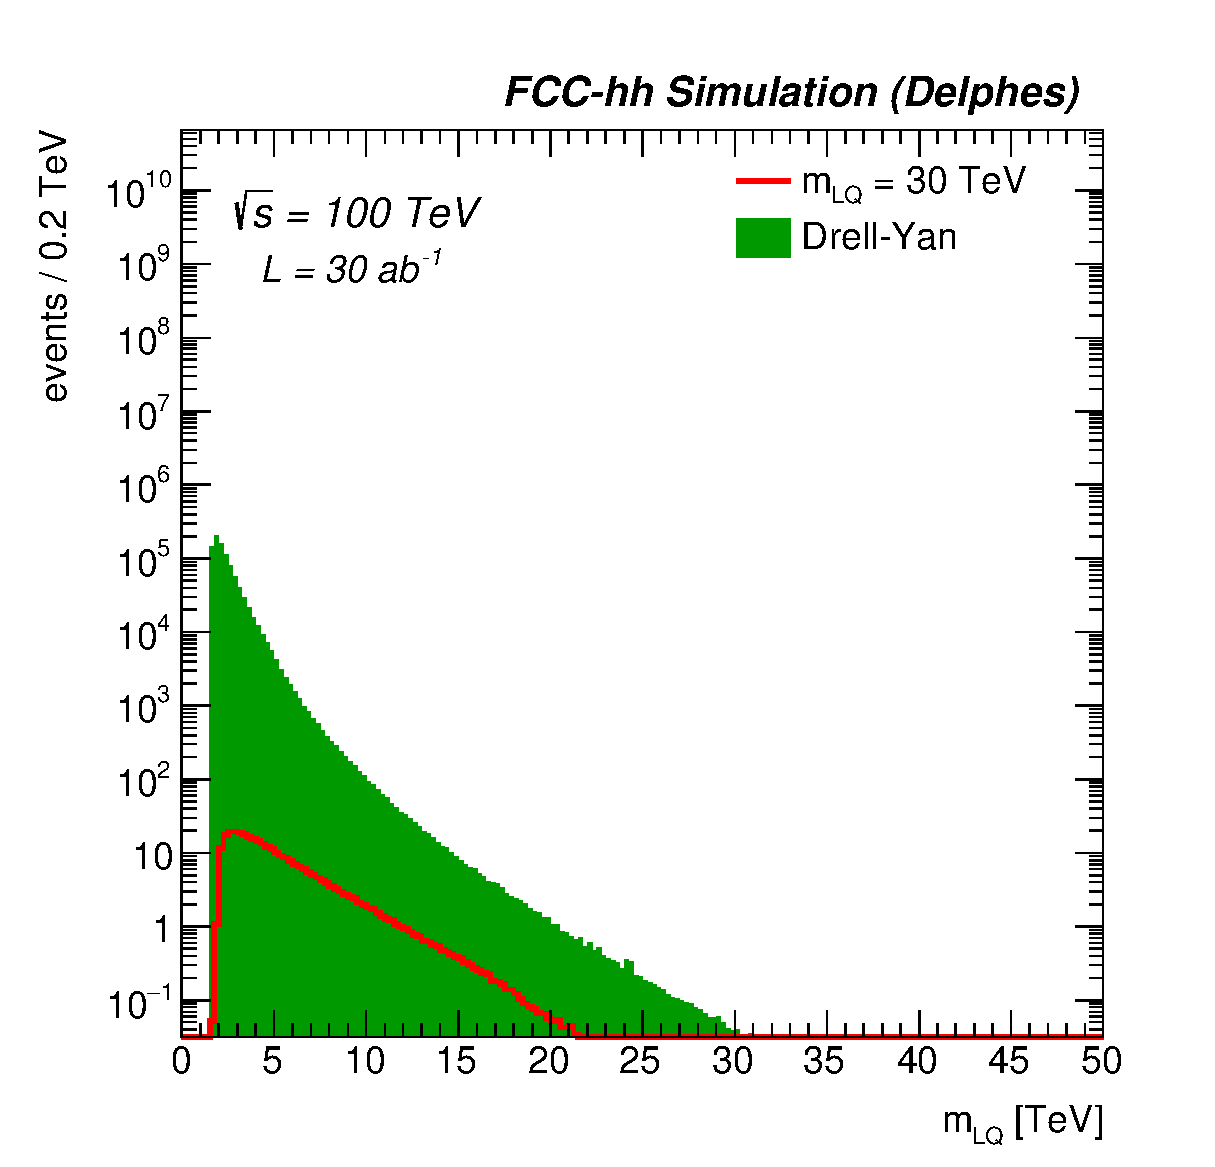
\includegraphics[width=0.32\columnwidth]{Fig/mlq_sel0_nostack_log.eps}
  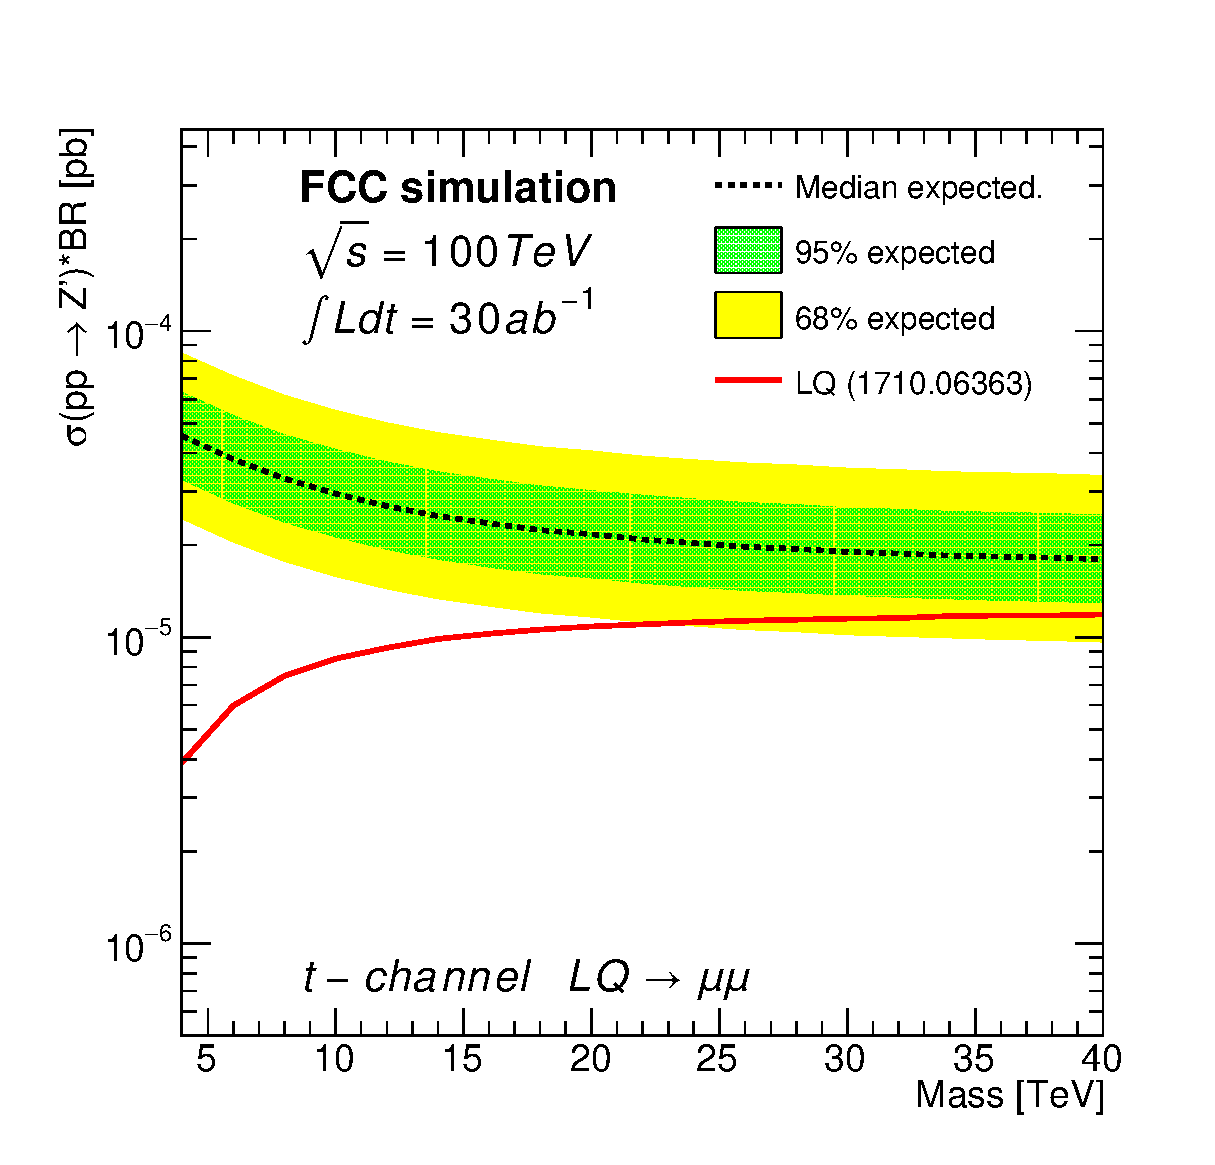
\includegraphics[width=0.32\columnwidth]{Fig/lim_LQ_mumu_fcc_v02.eps}
  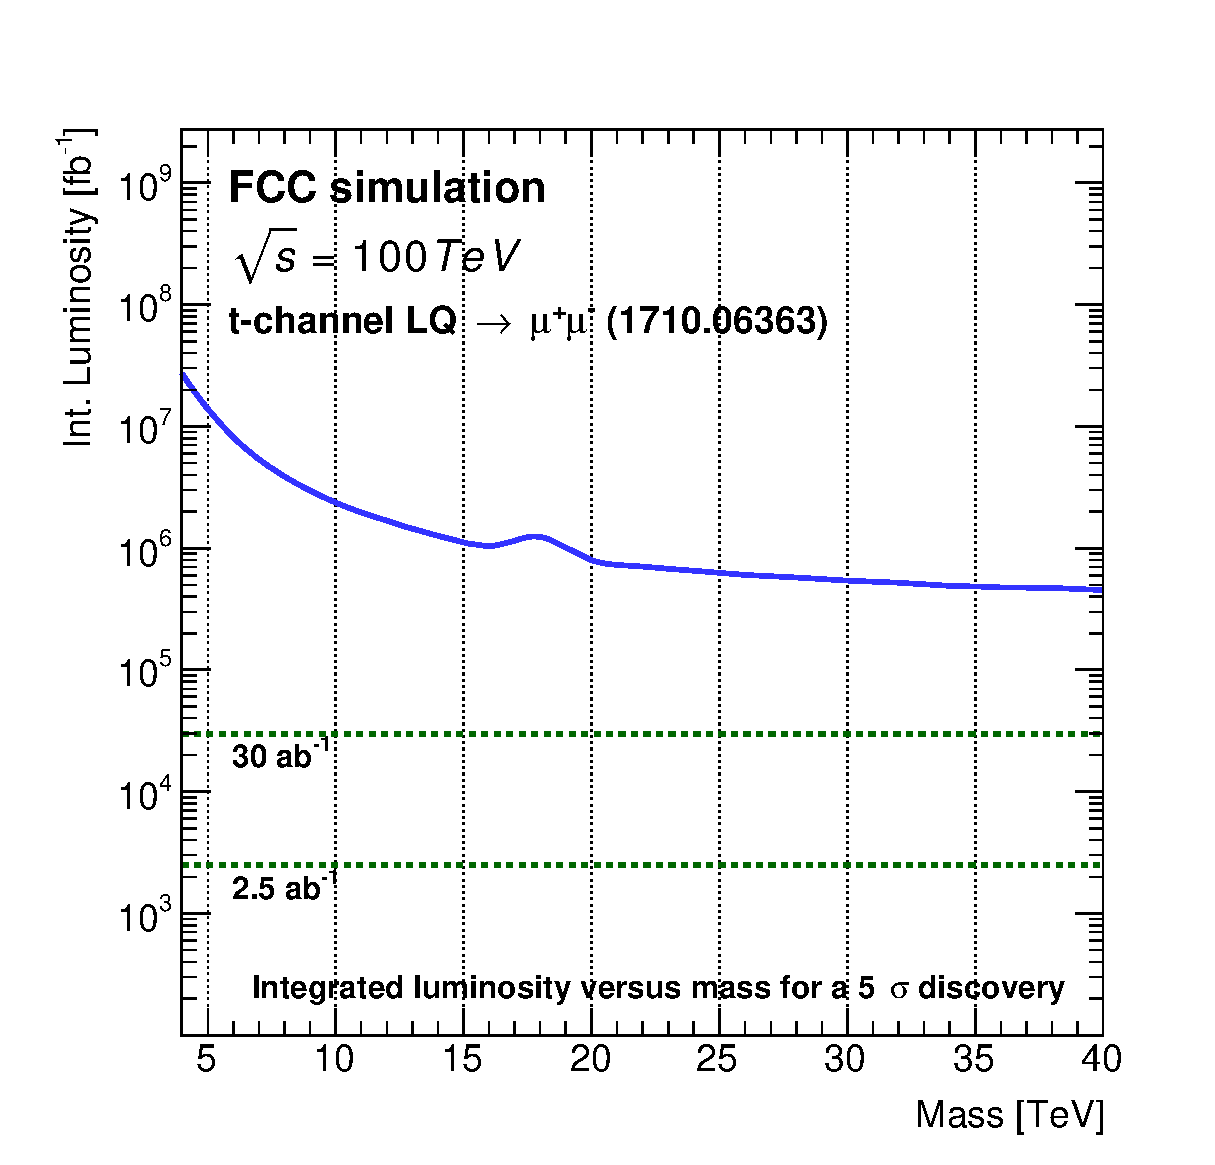
\includegraphics[width=0.32\columnwidth]{Fig/DiscoveryPotential_LQ_mumu_rootStyle.eps}
  \caption{Left : Invariant mass for a 30~TeV signal after full event selection in t-channel LQ scenario. Limit versus mass (middle) and luminosity for a $5\sigma$ discovery (right) comparing ee,$\mu\mu$ and combined channels. }
  \label{figure:leptonicresonances:resultsmumu_lq}
\end{figure}

\clearpage
\newpage

%%%%%%%%%%%%%%%%%%%%%%%%%%%%%%%%%%%%%%%%%%%%%%%%%%%%%
%%%%%%%%%%%%%%%%%%%%%%%%%%%%%%%%%%%%%%%%%%%%%%%%%%%%%
\subsection{Hadronic resonances : WW, \texorpdfstring{$t\bar{t}$}{tt}, jj}
\label{subsec:hadreso}

\subsubsection{Introduction}
Many models of beyond the SM (BSM) physics predict additional particles with masses at the TeV scale. The presence of new resonant states~\cite{Harris:2011bh,Boelaert:2009jm,Lee:1973iz,Branco:2011iw,Hill:1994hp,Kaplan:1983sm,Bellazzini:2014yua,Randall:1999ee,Pomarol:1999ad,Davoudiasl:1999tf} decaying to two highly boosted particles decaying hadronically could be observed as an excess in the QCD dijet distribution. We focus here on three specific benchmark models: a \ZpSSM~\cite{Langacker:2008yv}, a Randall-Sundrum graviton~\cite{Randall:1999ee}, and an excited quark resonance~\cite{Baur:1987ga,Baur:1989kv}. We study the sensitivity in the following decay using hadronic decay modes: \zptt, \rsg\ and \qjj.

The decay products are typically in the multi-TeV regime and their reconstruction imposes stringent requirement on the detector design. Precise jet energy resolution requires full longitudinal shower containment. Highly boosted top quarks and $W$ bosons decay into highly collimated jets that need to  be disentangled from standard QCD jets by studying their substructure. High discrimination power and sensitivity for these searches at such extreme energies, requires excellent granularity both in the tracking detectors and calorimeters.

%%%%%%%%%%%%%%%%%%%%%%%%%%%%%%%%%%%%%%%%%%%%%%%%%%%%%%%%%%%%%%%%%%%%%%%%%%%%%%%%%%%%%%%%%%%%
\subsubsection{Event Selection}

\subparagraph{Dijet analysis}

Jets are clustered using particle-flow candidates with the anti-$k_T$~\cite{Cacciari:2008gp} algorithm with parameter R=0.4. We require at least two jets with $\pt$>3~TeV and $|\eta<3|$ and the rapidity difference between the two leading jets to be small, $\Delta(\eta)<1.5$ as di-jet events will tend to be more central. The dijet invariant mass of the \qjj\ signal for $m_Q^{*}$ and QCD contributions after the full event selection is shown in Figure~\ref{figure:hadronicresonances:ttsel08} (left).

\subparagraph{Boosted Top and W analyses}

As track jets are better able to resolve the jet sub-structure compared to particle-flow jets, the jet selection for the \rsg\ and \zptt\ searches using track jets. As no lepton veto is applied, there is also some acceptance for leptonic decays. The sensitivity to semi-leptonic $WW$ or \ttbar\ decays is enhanced by adding the $\metvec$ vector to the closest jet 4-momentum (among the to leading jets).

We require two jets with a $\pt$>3~TeV and $|\eta<3|$ and $\Delta(\eta)<2.4$. Both jets must either be $W$ or top tagged (section~\ref{subsec:mvatagger}) by requiring multivariate tagger > 0.15. Both high-\pt\ jets must be $b$-tagged for the \zptt\ analysis. Finally, to further reject QCD, we require for both jets $m_{SD}>40$~GeV. In Figure~\ref{figure:hadronicresonances:ttsel08} we show the di-jet invariant mass distribution after the final cuts for the \rsg\ (center) and \zptt\ (right) analyses respectively.
\newline
More detailed results can be found in Appendix~\ref{appendix:zptt100} (\zptt) and~\ref{appendix:rsg100} (\rsg).

\begin{figure}[!htb]
  \centering
  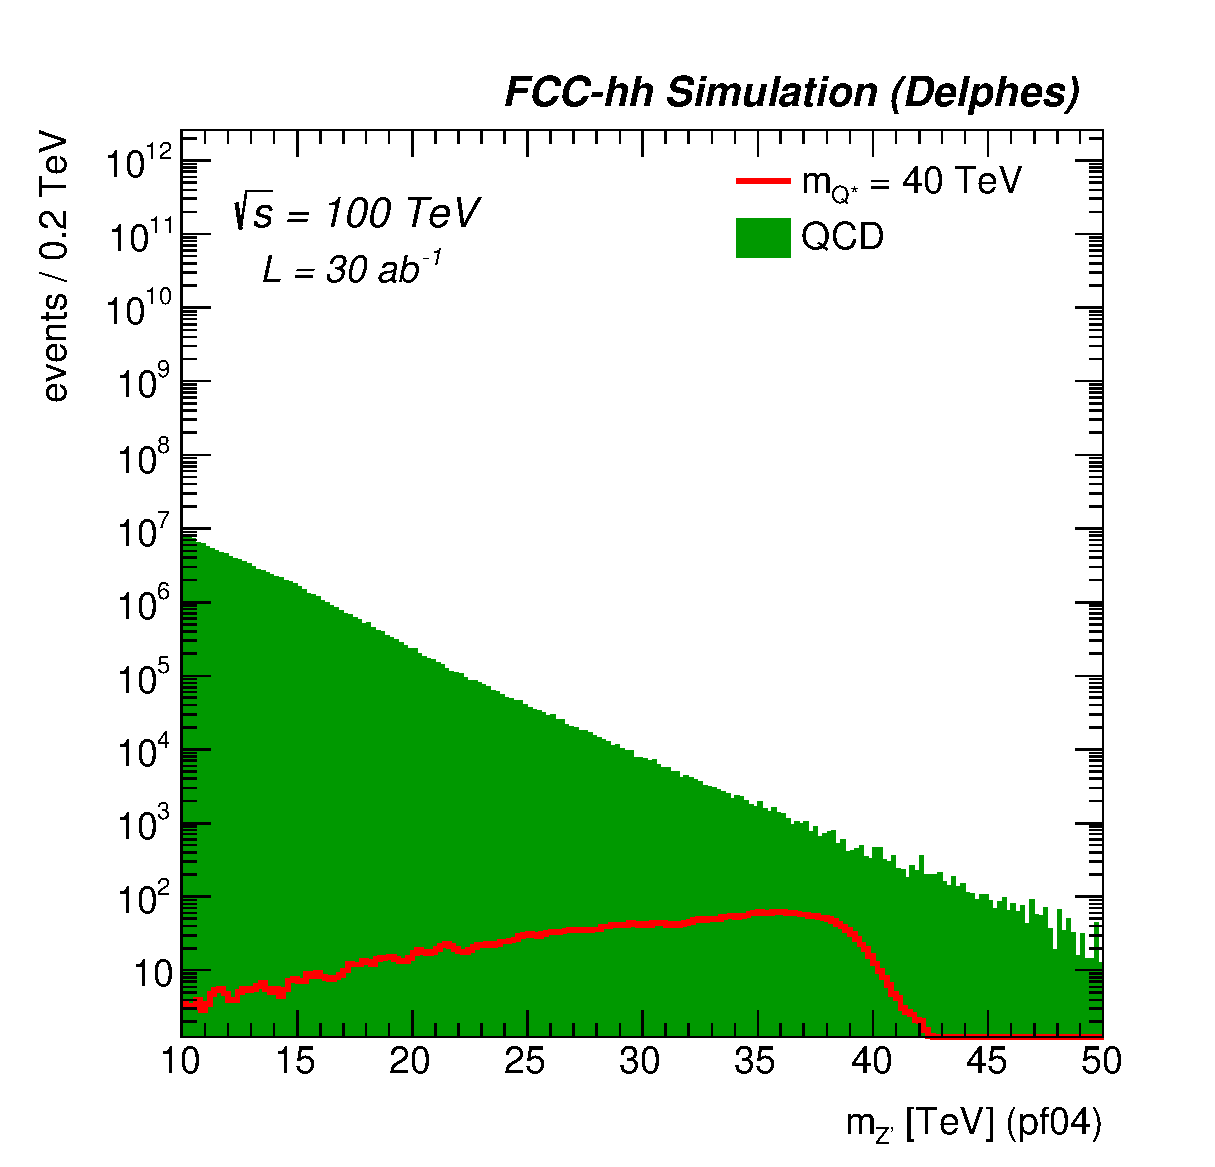
\includegraphics[width=0.32\columnwidth]{Fig/Mj1j2_pf04_sel1_nostack_log.eps}
  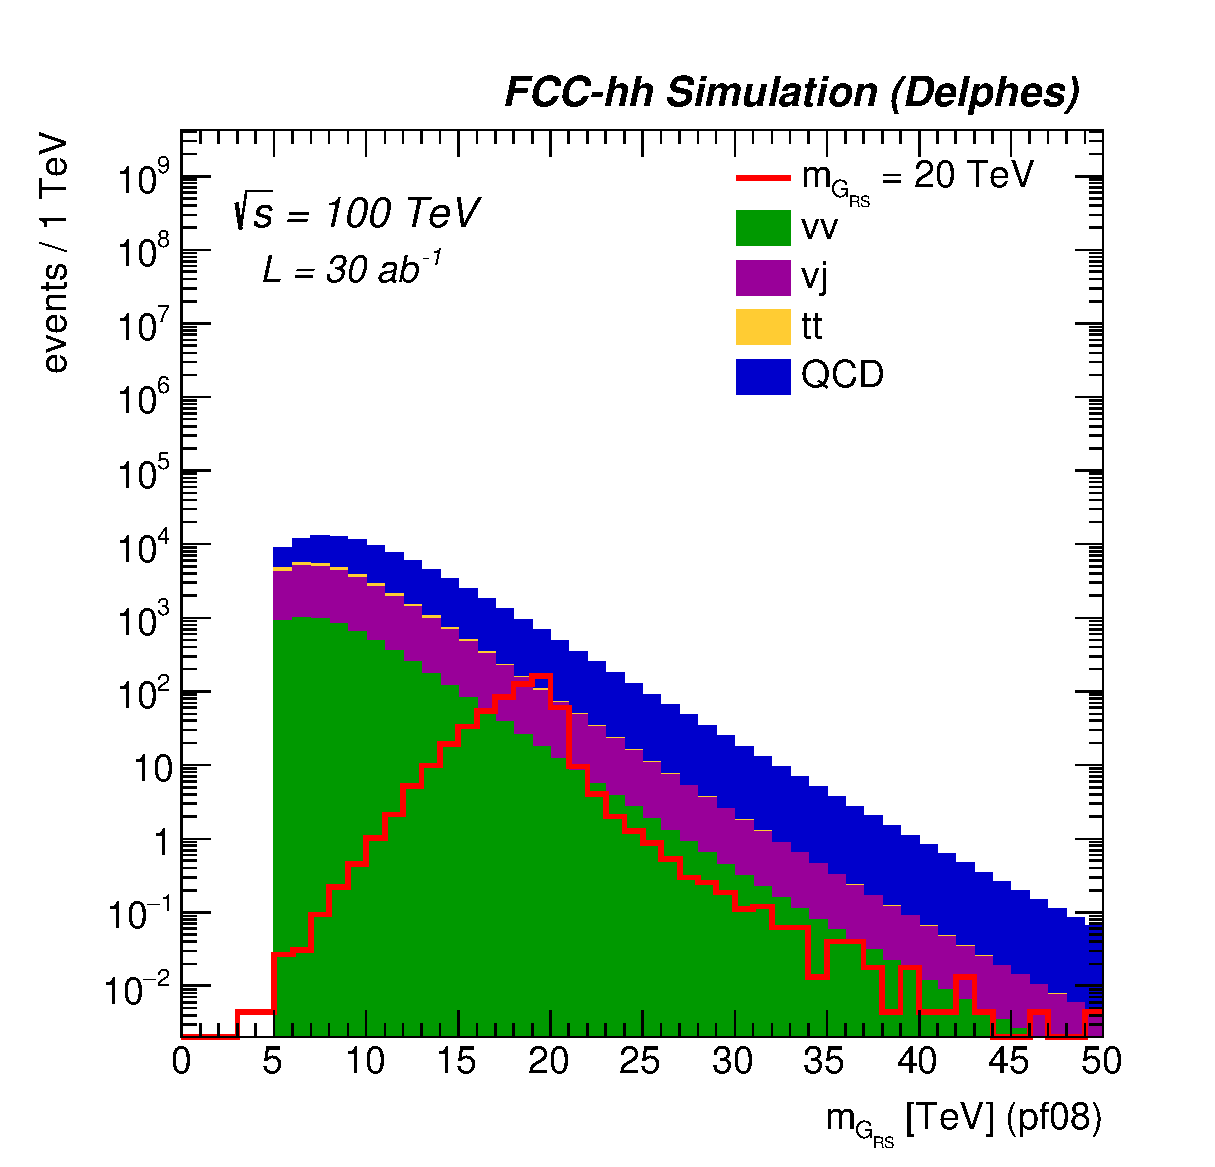
\includegraphics[width=0.32\columnwidth]{Fig/Mj1j2_pf08_fit_sel4_nostack_log.eps}
  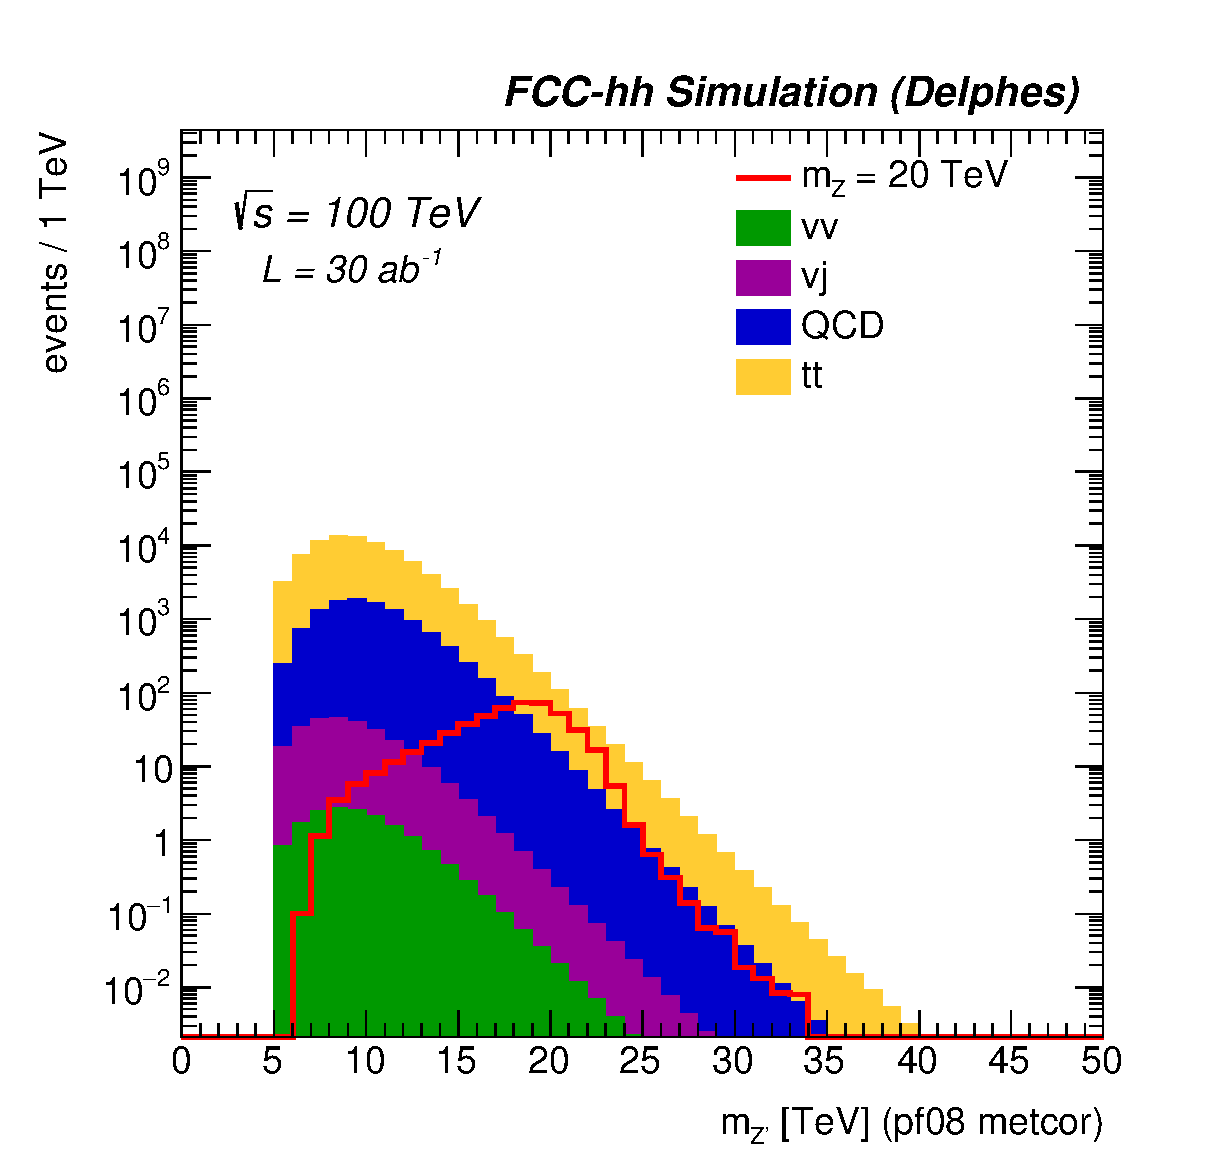
\includegraphics[width=0.32\columnwidth]{Fig/Mj1j2_pf08_MetCorr_fit_sel8_nostack_log.eps}
  \caption{Invariant mass distribution of the two leading jets for the pre-selection (left) and full selection (right) for a 40~TeV signal for the \qjj\ (left), and a 20~TeV signal for \rsg\ (center) and \zptt\ (right) analyses.\MS{need editing / style}}
  \label{figure:hadronicresonances:ttsel08}
\end{figure}

\begin{table}[htbp]
   \centering
\begin{tabular}{|c|c|c|c|c|c|c|c|c|}
  \hline
  \hline
  & \multicolumn{2}{c|}{di-jet}  & \multicolumn{2}{c|}{$\ttbar$} & \multicolumn{2}{c|}{WW} \\
  \cline{2-7}

 & pre-sel & final-sel  & pre-sel & final-sel & pre-sel & final-sel\\
  \hline
  di-jet & 385555434 &  373661126 &  154855591 & 11439.8&  154856148 & 64484\\
  $\ttbar$ & - & - & 1114779 & 74193.6 &  1114779 & 3185\\
  di-bosons & - & - &  41820 &  17.1 &  41820 & 6092\\
  boson+jet & - & - & 1610472 & 264.1&  1610472 & 25377\\
  \hline
  total bkg  &  385555434& 373661126& 157622662 & 85914 & 154856148 & 99137\\
  \hline
  10~TeV &  - & - &  101529 & 15601 &  47853 & 15745\\
  20~TeV &   1253072 &  1239813& 7774 & 500.6 & 1282 & 578\\
  30~TeV &  69922 &  67488 & 485.2 & 13.2 &  61.4 & 30.1 \\
  40~TeV &  4589 &  4373 & - & - & - & -\\
  \hline
  \hline
\end{tabular}
  \caption{Yields for the di-jet, $\ttbar$ and WW analyses after pre and final selection.}
  \label{tab:hadronicresonances:yields}
\end{table}

%%%%%%%%%%%%%%%%%%%%%%%%%%%%%%%%%%%%%%%%%%%%%%%%%%%%%%%%%%%%%%%%%%%%%%%%%%%%%%%%%%%%%%%%%%%%
\subsubsection{Signal extraction and results}
Hypothesis testing is performed using a modified frequentist method based on a profile likelihood fit that takes into account the systematic uncertainties as nuisance parameters. The di-jet invariant mass is used as a discriminant. In order to reduce large statistical fluctuations from high Monte Carlo weight events, we parameterize the background invariant mass distribution with the following function (conservatively assuming 50\% uncertainty on the background normalisation) $f(z)=p_1(1-z)^{p_2}z^{p_3}z^{p_{4}logz}$, where $z=m_{jj}/\sqrt{s}$.

The expected exclusion limits at 95\% CL are shown in Figures~\ref{figure:hadronicresonances:limits} and~\ref{figure:hadronicresonances:resultsjj}. For the \qjj\ masses up to 40~TeV could be discovered with \intlumifcc. Reconstructing Heavy resonances decaying to $WW$ and \ttbar\ is more challenging and requires the use of novel approaches to boosted object tagging to reduce the backgrounds. The reach for \zptt\ (in TC2 models) and \rsg\ is 24~TeV and 22~TeV respectively and it is possible to discover a $Z^{\prime}_{SSM} \rightarrow \ttbar$ up to $m_{Z}=18$~TeV.

\begin{figure}[!htb]
  \centering
  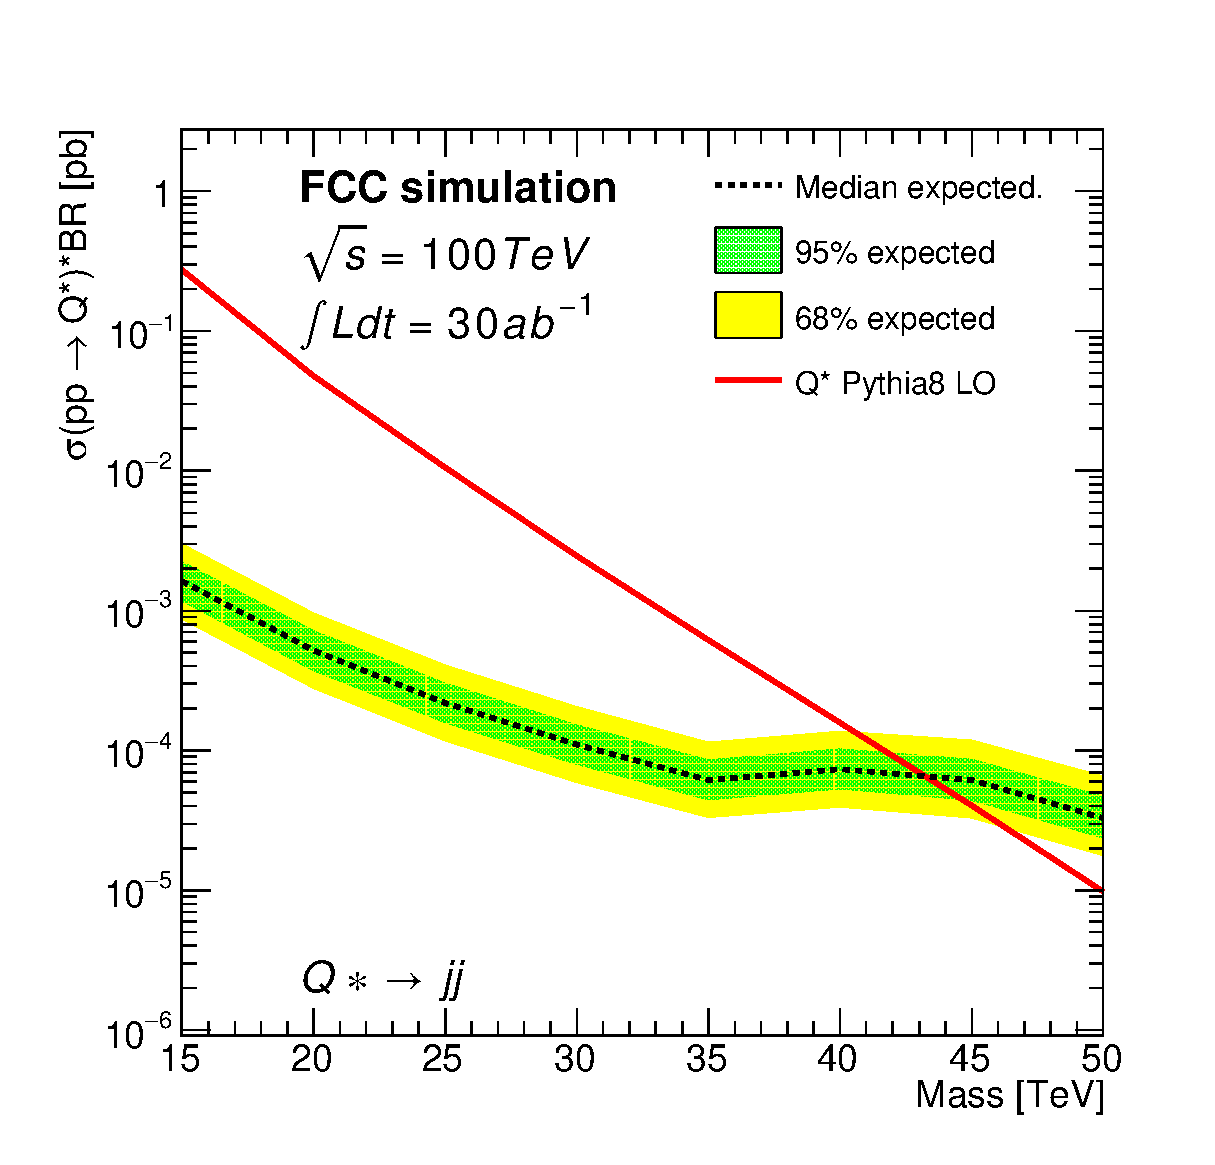
\includegraphics[width=0.30\columnwidth]{Fig/lim_Qstar_jj_fcc_v02.eps}
  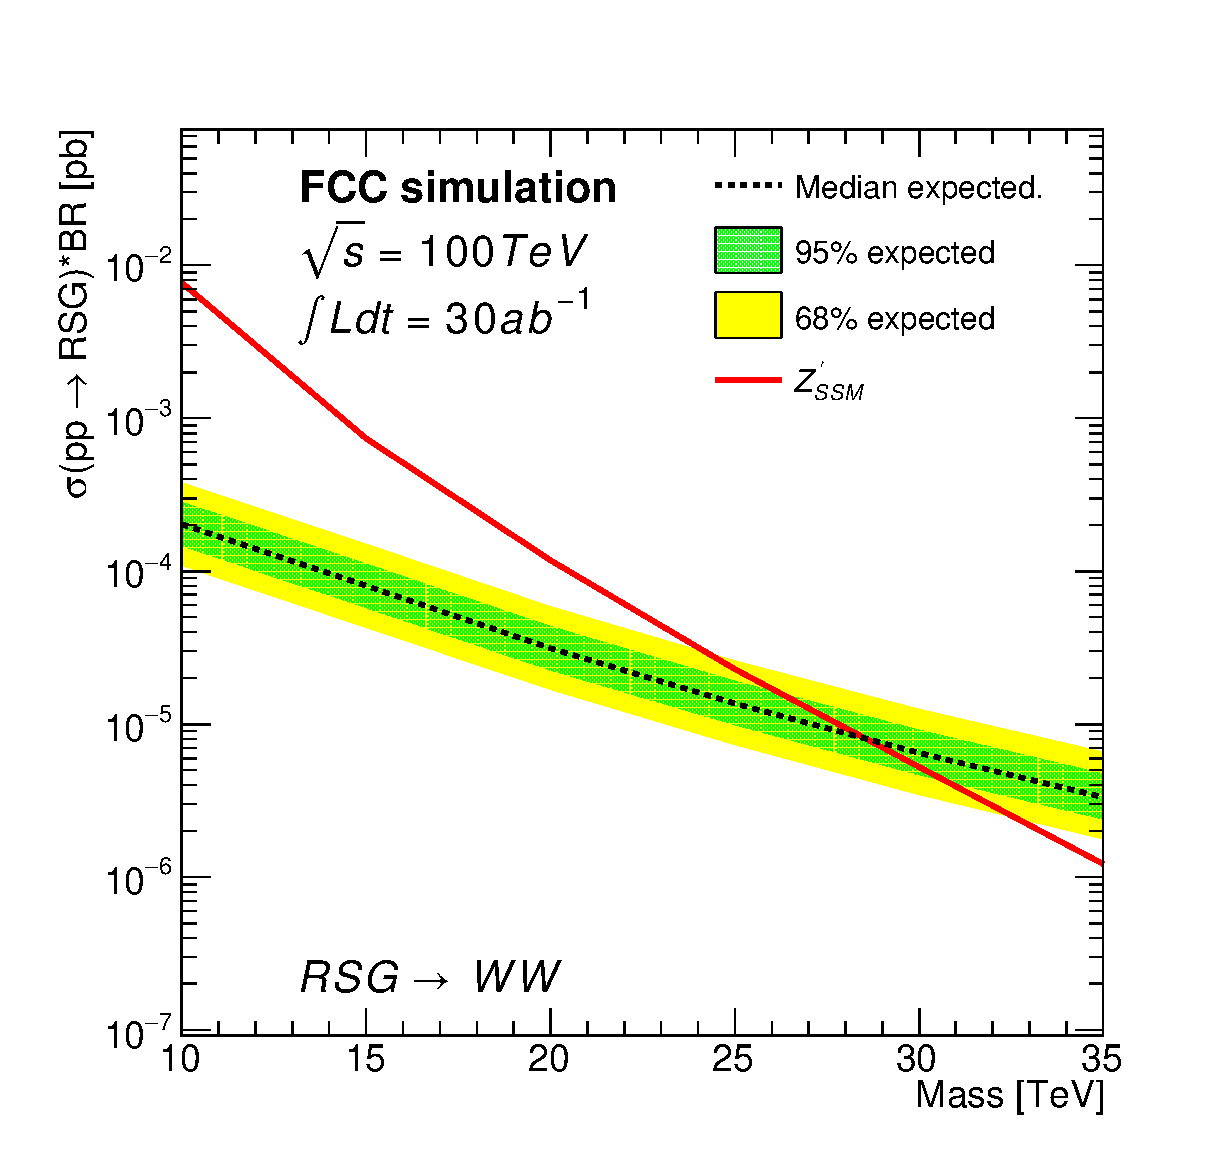
\includegraphics[width=0.30\columnwidth]{Fig/lim_RSGraviton_ww_fcc_v02.eps}
  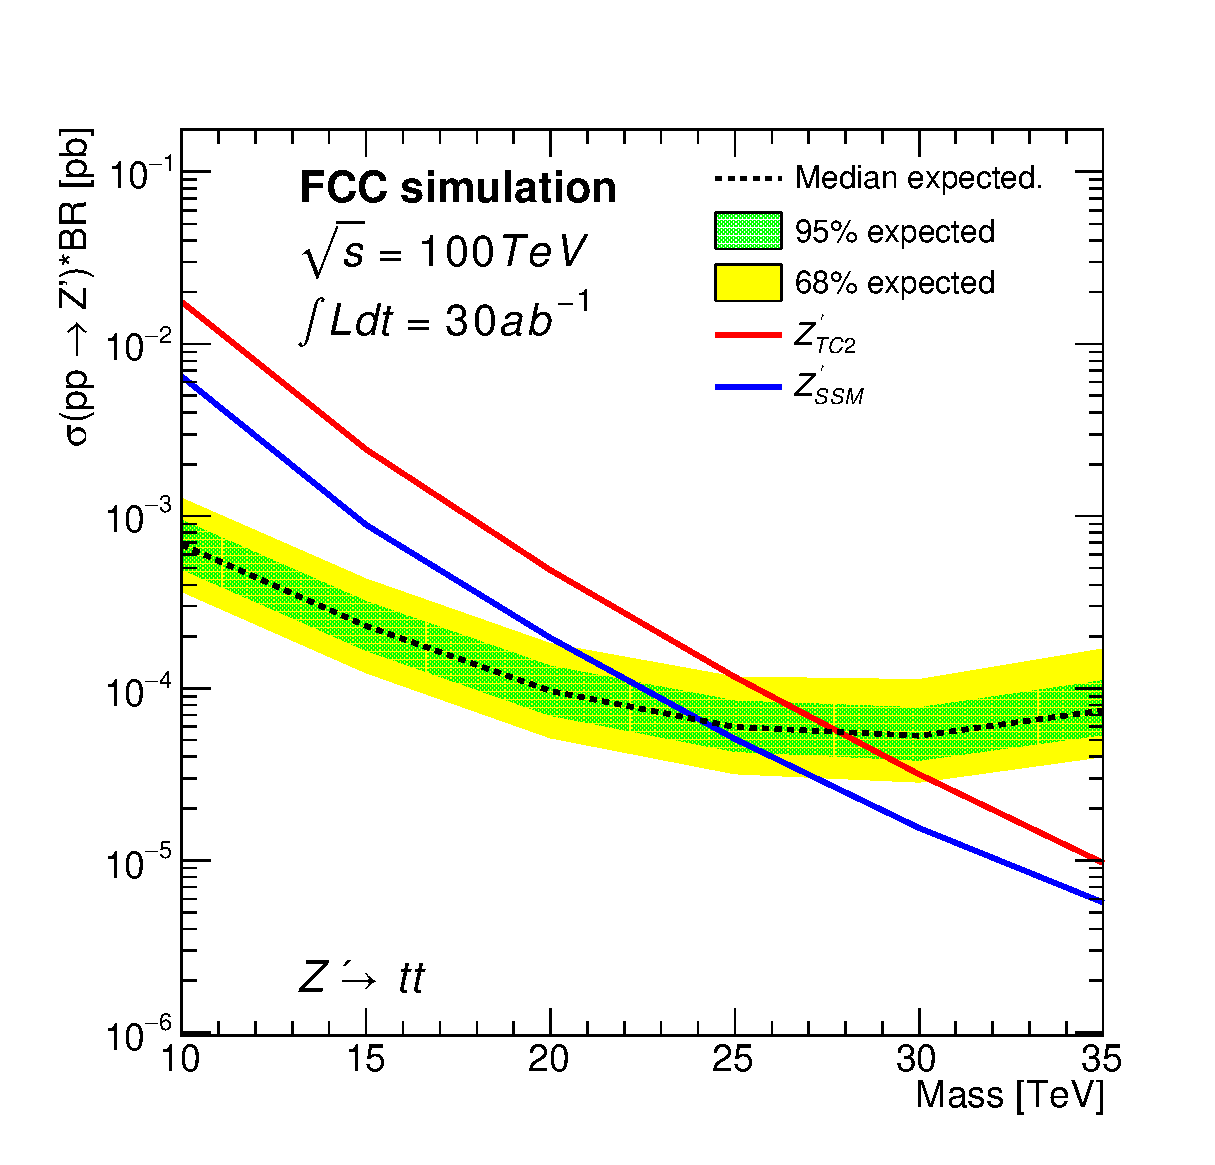
\includegraphics[width=0.30\columnwidth]{Fig/lim_Zprime_tt_fcc_v02.eps}
  \caption{Exclusion limit at 95\% CL versus heavy resonance mass decaying into di-jet (left), WW (center), \ttbar\ (right).}
  \label{figure:hadronicresonances:limits}
\end{figure}

\begin{figure}[!htb]
  \centering
  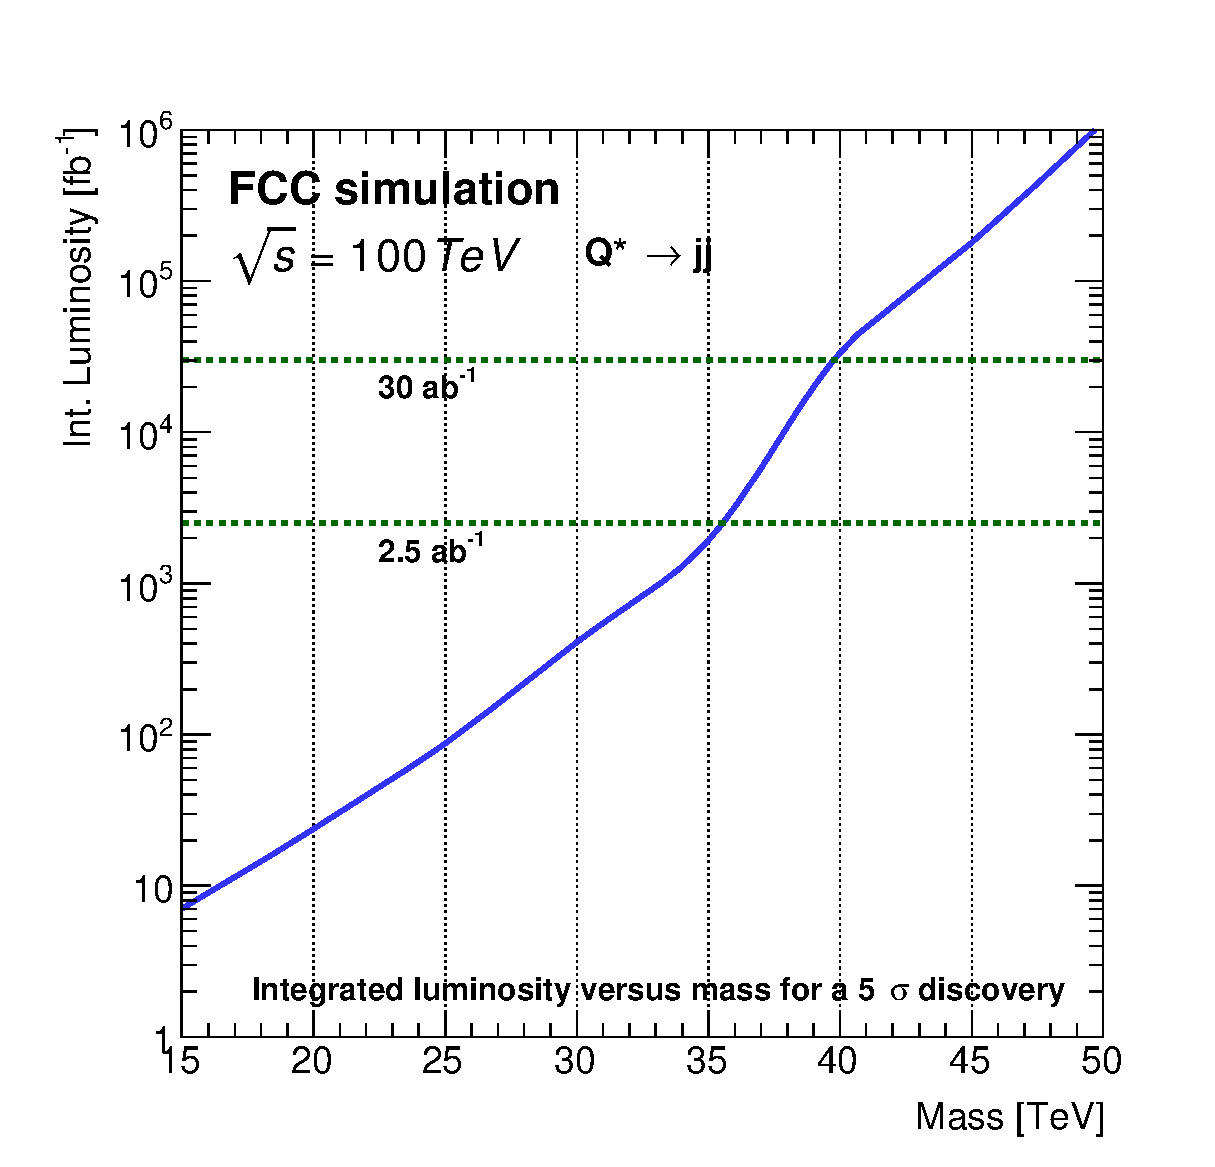
\includegraphics[width=0.30\columnwidth]{Fig/DiscoveryPotential_jj_rootStyle.eps}
  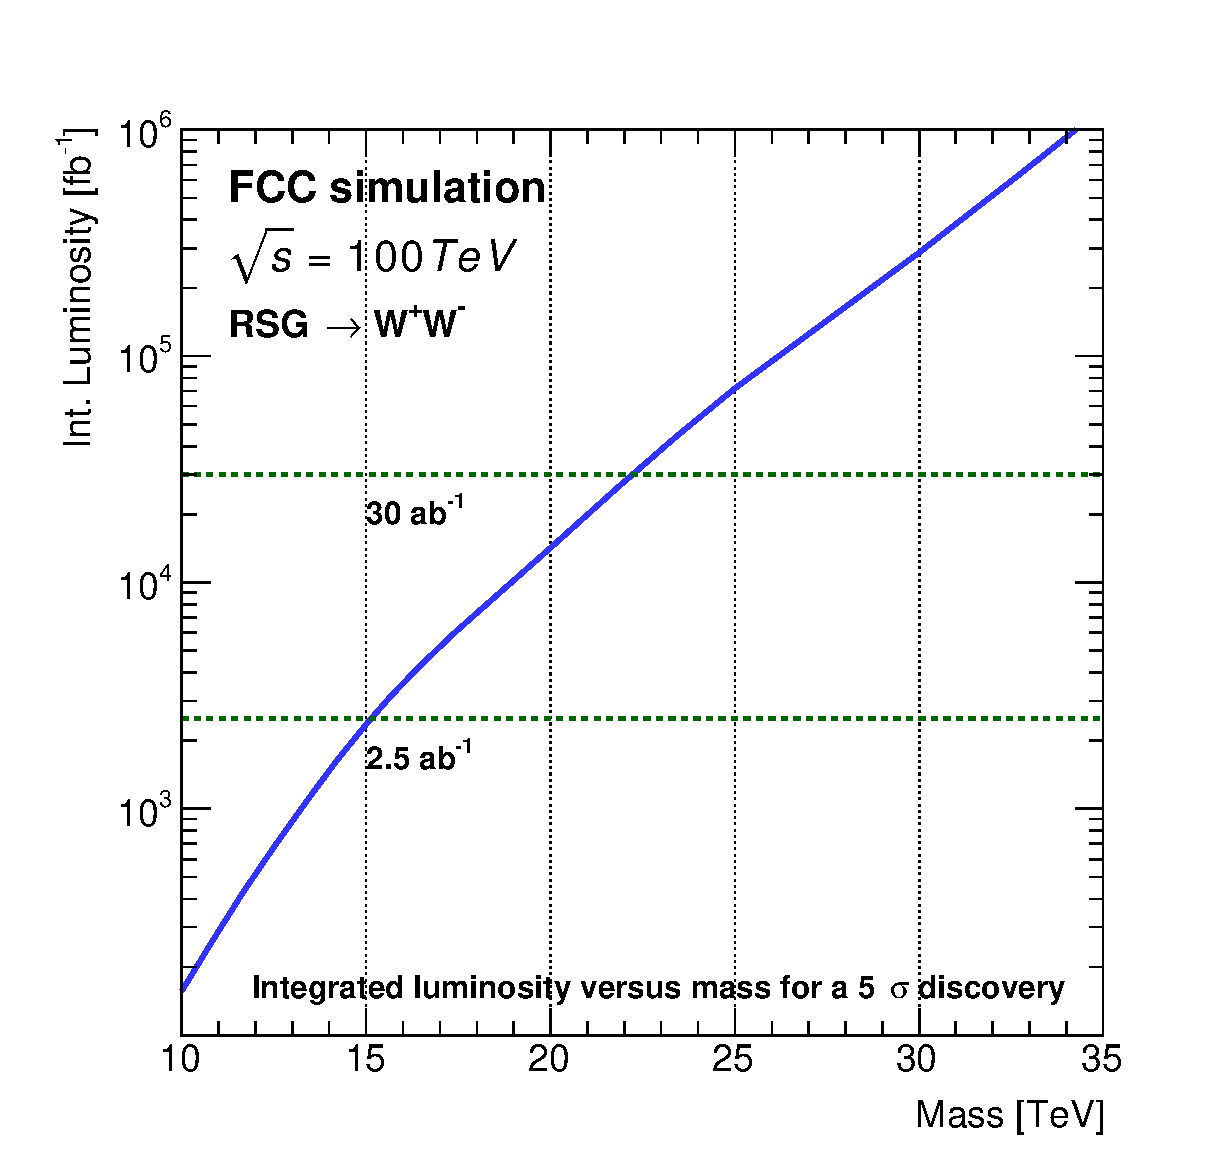
\includegraphics[width=0.30\columnwidth]{Fig/DiscoveryPotential_ww_tagger_rootStyle.eps}
  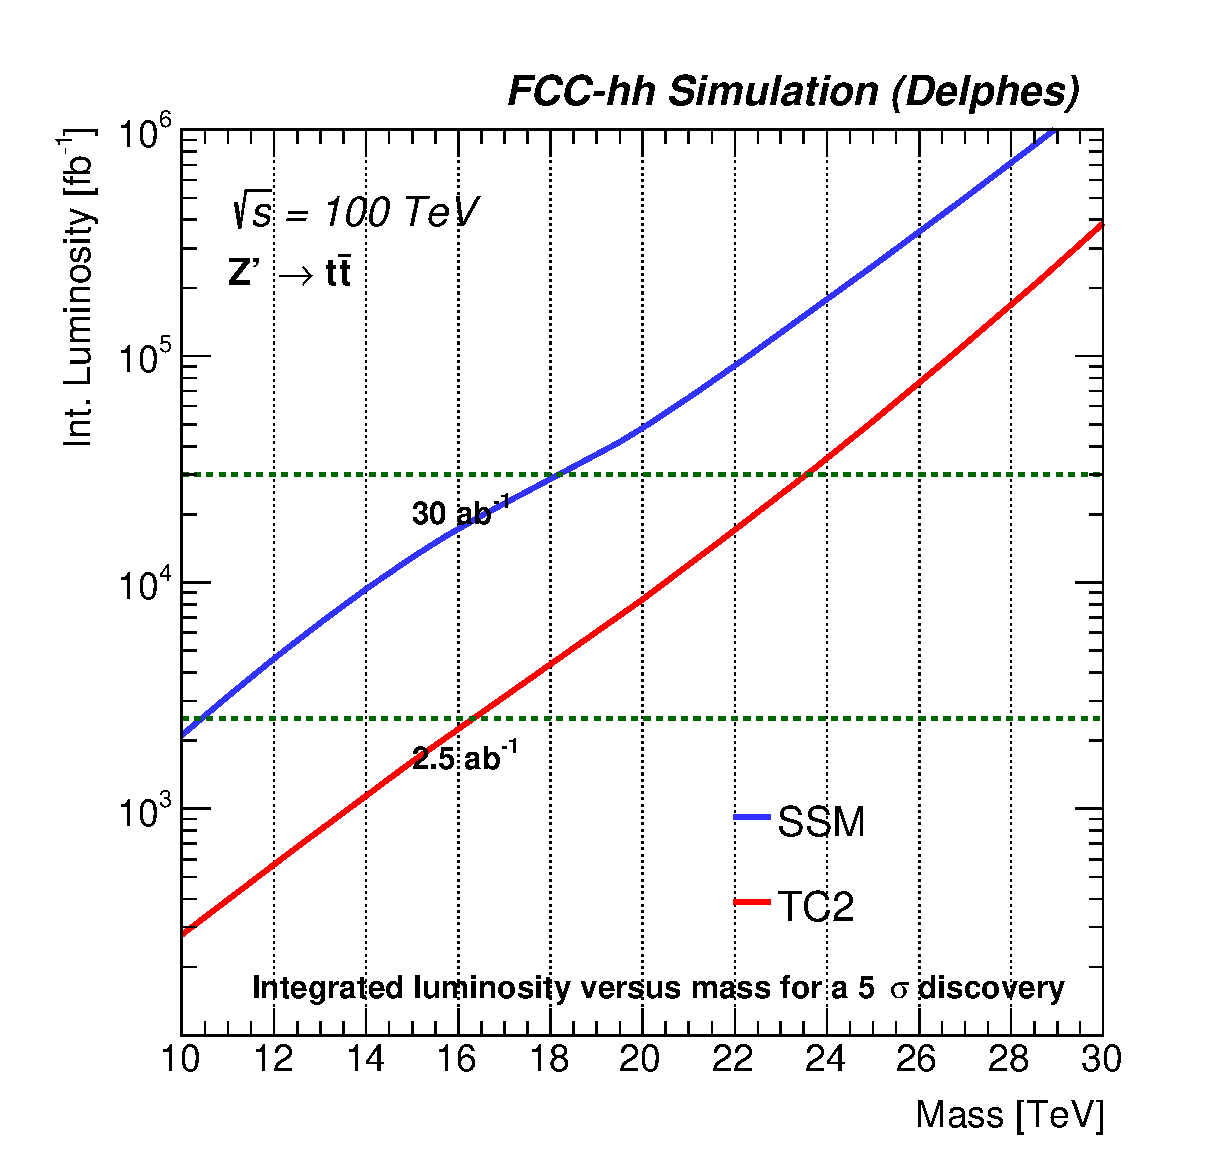
\includegraphics[width=0.30\columnwidth]{Fig/DiscoveryPotential_tt_SSM_TC2_tagger_TRFbtag_rootStyle.eps}
  \caption{Integrated luminosity for a $5\sigma$ discovery as a function of the heavy resonance mass decaying into di-jet (left), WW (center), \ttbar\ (right).}
  \label{figure:hadronicresonances:resultsjj}
\end{figure}

\clearpage
\newpage
